\documentclass[12pt,a4paper]{article}
\usepackage{tikz}
\usetikzlibrary{arrows}
\usepackage{latexsym}
\usepackage{tech,mathsx}
\usepackage{cspm}
\usepackage{scalalistings}

\newtheorem{lemma}{Lemma}
\newtheorem{definition}[lemma]{Definition}
\newtheorem{prop}[lemma]{Proposition}

\def\s#1{$_{#1}$}
\def\call{\mathsf{call}}
\def\return{\mathsf{return}}
\def\::{\mathord{\hspace{0.1mm}:\hspace{0.1mm}}}
\def\range#1#2{[#1 \mathbin{..} #2)}
\def\op{{\sm{op}}}
\def\sync{\sm{sync}}
\def\send{\sm{send}}
\def\receive{\sm{receive}}

% tikz stuff

\def\X{node {$\cross$}}
% Bullet at (#1,#2) with text #3 below
\def\bulletAt(#1,#2)#3{%
  \draw(#1,#2) node {$\bullet$}; \draw(#1,#2-0.4) node{\footnotesize #3};
}
% Cross at (#1,#2) with text #3 below
\def\crossAt(#1,#2)#3{%
  \draw(#1,#2) \X; \draw(#1,#2-0.4) node{\footnotesize #3};
}

\def\topfraction{0.75}
\renewcommand{\floatpagefraction}{0.7}

\sloppy\raggedbottom

\title{Understanding Synchronisation}
\author{Jonathan Lawrence and Gavin Lowe}

\begin{document}
\maketitle

\begin{abstract}
\ldots
\end{abstract}

%%%%%%%%%%%%%%%%%%%%%%%%%%%%%%%%%%%%%%%%%%%%%%%%%%%%%%%

\begin{frontmatter}
\title{Synchronisation: Specification and Testing}

\author{Jonathan Lawrence}
\ead{jonathan@tbtl.com}
\affiliation{organization = {The Blockhouse Technology Ltd.}, city = {Oxford},
  country = {UK}}

\author{Gavin Lowe\corref{cor1}}
\ead{gavin.lowe@cs.ox.ac.uk} 
\affiliation{organization = {St Catherine's College, University of
    Oxford}, country = {UK}}
\cortext[cor1]{Corresponding author.}

\journal{Science of Computer Programming}

\begin{abstract}
We study \emph{synchronisation objects}: objects that allow two or more
threads to synchronise, each waiting until the other threads have reached a
particular point, and maybe exchanging data.  We define a correctness
condition for such synchronisation objects, which we call
\emph{synchronisation linearisation}: informally, the synchronisations appear
to take place in a one-at-a-time order, consistent with the calls and returns
of operations on the object, and giving correct results.  We also define a
liveness condition, which we call \emph{synchronisation progressibility}:
informally, executions of operations don't get stuck when a synchronisation is
possible.  We show that synchronisation linearisation can be reduced to a
variant of standard linearisation, which we call \emph{two-step
  linearisation}, where each operation of the synchronisation object is
linearised in \emph{two} steps.

We consider testing of implementations of synchronisation objects.  The basic
idea is to run several threads that use the object, record the history of
operation calls and returns, and then test whether the resulting history
satisfies synchronisation linearisation and progressibility.  We present
algorithms for this last step, and give results concerning the complexity of
the problem.  We describe an implementation of such a testing framework, and
present experimental results.
\end{abstract}

\begin{keyword}
Concurrent programming \sep
synchronisation \sep specification \sep linearisation \sep synchronisation
linearisation \sep synchronisation progressibility \sep two-step linearisation
\sep testing.
\end{keyword}
\end{frontmatter}

%%%%%%%%%%%%%%%%%%%%%%%%%%%%%%%%%%%%%%%%%%%%%%%%%%%%%%%

\section{Introduction}

In many concurrent programs, it is necessary at some point for two or more
threads to \emph{synchronise}: each of the threads waits until the other
threads have reached a particular point before continuing; in addition, the
threads can exchange or combine data.  Reasoning about programs can be easier
when synchronisations are used: it helps to keep threads in consistent stages
of the program, and so makes it easier to reason about the states of different
threads. (The word ``synchronisation'' is used in a couple of different ways
within concurrent programming: we use it in the sense just described, where
every thread waits for the others, rather than for more general coordination
between threads, such as via a semaphore which allows asynchrony between a
signal and the receipt of the signal.)

We study synchronisations in this paper: we describe how synchronisations can
be specified, and what it means for such a specification to be satisfied.  We
also describe techniques for testing implementations. 

We start by giving some examples of synchronisations in order to illustrate
the idea.  (We use Scala notation; we explain non-standard aspects of the
language in footnotes.)  In each case, the synchronisation is mediated by a
\emph{synchronisation object}.

Perhaps the most common form of synchronisation object is a synchronous
channel, e.g.~\cite{H78,occam,andrews,JCSP,sufrin:CSO,DK-go}.  Such a channel
might have signature\footnote{The class is polymorphic in the
  type~{\scalashape A} of data.  The type {\scalashape Unit} is the type that
  contains a single value, the \emph{unit value}, denoted~{\scalashape ()}.}
%
\begin{scala}
class SyncChan[A]{
  def send(x: A): Unit
  def receive(): A
}
\end{scala}
%
Each execution of one of the operations must synchronise with an execution
of the other operation: the two executions must overlap in time.  If an
execution |send(x)| synchronises with an execution of |receive|, then the
|receive| returns~|x|.

Each synchronisation of a synchronous channel involves executions of two
\emph{different} operations (|send| and |receive|); we say that the
synchronisation is \emph{heterogeneous}.  By contrast, sometimes two
executions of the \emph{same} operation may synchronise; we say that the
synchronisation is \emph{homogeneous}.  For example, an
\emph{exchanger}~\cite{HSY2004,herlihy-shavit} has the following signature:
%
\begin{scala}
class Exchanger[A]{
  def exchange(x: A): A
}
\end{scala}
%
When two threads call |exchange|, the executions can synchronise, and each
receives the value passed in by the other.

For some synchronisation objects, synchronisations might involve more than two
threads.  For example, a \emph{barrier synchronisation}
object~\cite{andrews,JCSP,SCL} can be used to synchronise~|n| threads:
%
\begin{scala}
class Barrier(n: Int){
  def sync(me: Int): Unit
}
\end{scala}
%
Each thread is assumed to have an integer thread identifier in the range
$\range{0}{\sm{n}}$.  Each thread~|me| calls |sync(me)|, and no execution
returns until all~|n| have called it.  We say that the synchronisation has
\emph{arity}~|n|.

A \emph{combining barrier}~\cite{andrews,SCL}, in addition to acting as a barrier
synchronisation, also allows each thread to submit a parameter, and for all to
receive back some function of those parameters.\footnote{The Scala type
  {\scalashape (A,A) =}$>$ {\scalashape A} represents functions from pairs of
  {\scalashape A} to~{\scalashape A}.}
%
\pagebreak[3]
%\begin{samepage}
\begin{scala}
class CombiningBarrier[A](n: Int, f: (A,A) => A){
  def sync(me: Int, x: A): A
}
\end{scala}
%\end{samepage}
%
The function |f| is assumed to be associative.  If |n| threads call |sync|
with parameters $x_1, \ldots, x_{\ss n}$, in some order, then each receives
back $\sm f(x_1, \sm f(x_2, \ldots \sm f(x_{{\ss n}-1}, x_{\ss n}) \ldots ))$.
(In the common case that |f| is commutative, this result is independent of the
order of the parameters.)

Some synchronisation objects have multiple modes of synchronisation.  For
example, consider a synchronous channel with timeouts: each execution might
synchronise with another execution, or might timeout without
synchronisation~\cite{sufrin:CSO,SCL}.  Such a channel has a signature as
follows.
%
\begin{scala}
class TimeoutChannel[A]{
  def send(x: A): Boolean
  def receive(): Option[A]
}
\end{scala}
%
The |send| operation returns a boolean to indicate whether the send was
successful, i.e.~whether it synchronised.  The |receive| operation can return
a value |Some(x)| to indicate that it synchronised and received~|x|, or can
return the value |None| to indicate that it failed to synchronise\footnote{The
  type {\scalashape Option[A]} contains the union of such values.}.  Thus an
execution of each operation may or may not synchronise with an execution of
the other operation.  Unsuccessful executions of |send| and |receive|
can be considered \emph{unary} synchronisations.  

Similarly, a timeout exchanger~\cite{HSY2004,herlihy-shavit} can allow threads
to exchange; but if a thread fails to exchange, it can return without
synchronising.  It has a signature as follows.
\begin{scala}
class TimeoutExchanger[A]{
  def exchange(x: A): Option[A]
}
\end{scala}


So far, our example synchronisation objects have been \emph{stateless}: they
maintain no state from one synchronisation to another.  By contrast, some
synchronisation objects are \emph{stateful}: they maintain some state between
synchronisations, which might affect synchronisations.  As a toy example,
consider a synchronous channel that maintains a sequence counter, and such
that both executions receive the current value of this counter.
\begin{mysamepage}
\begin{scala}
class SyncChanCounter[A]{
  private var counter: Int
  def send(x: A): Int      // Result is sequence counter.
  def receive(): (A, Int)  // Result is (value received, sequence counter).
}
\end{scala}
\end{mysamepage}

% Variations: homogenous case; different modes

Some implementations of synchronous channels allow the channel to be
closed~\cite{JCSP,sufrin:CSO}, say by a unary operation |close|.
\begin{scala}
class CloseableChan[A]{
  def send(x: A): Unit
  def receive(): A
  def close(): Unit
}
\end{scala} 
%
Calls to |send| or |receive| after the channel is closed throw an exception.
Thus such an object is stateful, with two states, open and closed; and the
operations have different modes of synchronisation, either successful or
throwing an exception.

An \emph{enrollable barrier}~\cite{alting-barrier} is a barrier
that allows threads to enrol and resign (via unary operations):
%
\begin{scala}
class EnrollableBarrier(n: Int){
  def sync(me: Int): Unit
  def enrol(me: Int): Unit
  def resign(me: Int): Unit
}
\end{scala} 
%
Each barrier synchronisation is between all threads that are currently
enrolled, so |sync| has a variable arity.  The barrier has a state, namely the
currently enrolled threads.

A \emph{terminating queue} can also be thought of as a stateful
synchronisation object with multiple modes.  Such an object mostly acts like a
standard partial concurrent queue: if a thread attempts to dequeue, but the
queue is empty, it blocks until the queue becomes non-empty.  However, if a
state is reached where all the threads are blocked in this way, then they all
return a special value to indicate this fact.  In some concurrent algorithms,
such as a concurrent graph search, this latter outcome indicates that the
algorithm should terminate.  Such a terminating queue might have the following
signature, where a dequeue returns the value |None| to indicate the
termination case.
%
\begin{scala}
class TerminatingQueue[A](n: Int){ // £n£ is the number of threads   
  def enqueue(x: A): Unit
  def dequeue: Option[A]
}
\end{scala} 
%
The termination outcome can be seen as a synchronisation between all |n|
threads.  This terminating queue combines the functionality of a
concurrent datatype and a synchronisation object.


%% In general, a synchronisation will involve some number~$k$ of threads, calling
%% operations of the form
%% %
%% \begin{scala}
%%   def op£\s1£(x£\s1£: A£\s1£): B£\s1£
%%   ...
%%   def op£\s k£(x£\s k£: A£\s k£): B£\s k£
%% \end{scala}
%% %
%% Each thread passes in some data, and receives back a result. 

In this paper, we consider what it means for such a synchronisation
object to be correct.  We also present techniques for testing correctness of
implementations.

In Section~\ref{sec:spec} we describe how to specify a synchronisation object:
we call the property \emph{synchronisation linearisation}.  The definition has
similarities with that of
\emph{linearisation}~\cite{herlihy-wing,herlihy-shavit}.  Linearisation is the
standard correctness property for concurrent datatypes (by which we mean
implementations of abstract dataypes, such as sets, mappings, stacks and
queues, that support concurrent operations).  However, synchronisation
linearisation talks about synchronisations between executions of operations,
whereas linearisation talks about single executions.  Informally, the
synchronisations should appear to take place in a one-at-a-time order,
consistent with the calls and returns of operations on the synchronisation
object.
%%  and with results as defined by a \emph{synchronisation specification
%%   object}.
We present a way to specify what sequences of synchronisations and what
return values are consider correct, via a \emph{synchronisation specification
  object}.

In fact, our property of synchronisation linearisation turns out to be the
same as \emph{set linearisation}~\cite{Neiger-1994}, also known as
\emph{concurrency-aware linearisation}~\cite{HRV-2015}.  We compare these
approaches with our own in Section~\ref{sec:related}.  We prefer the name
``synchronisation linearisation'' here, because it best describes our
intention.

We also define a liveness condition, which we call \emph{synchronisation
  progressibility}: informally, executions don't get stuck when a
synchronisation is possible.

In Section~\ref{sec:relating} we consider the relationship between
synchronisation linearisation and (standard) linearisation.  We show that
linearisation is an instance of synchronisation linearisation, but that
synchronisation linearisation is more general.  We also show that
synchronisation linearisation corresponds to a small adaptation of
linearisation, where an operation of the synchronisation object may correspond
to \emph{two} operations of the object used to specify linearisation; we call
this \emph{two-step linearisation}.

We then consider testing of synchronisation object implementations.  Our
experience from teaching students is that they often do not have a clear idea
about how to test a synchronisation object (we suspect the same is true of
other programmers).  Yet, implementing synchronisation objects is
tricky---subtle bugs are fairly common---and so good tests are important.

Our testing techniques are based on the techniques for testing (standard)
linearisation~\cite{wing-gong,gavin:lin-testing}, which we review in
Section~\ref{sec:lin-testing}: the basic idea is to record a history of
threads using the object, and then to check whether that history is
linearisable.
%
In Section~\ref{sec:testing-hacking} we show how this technique can be adapted
to test for synchronisation linearisation, using the result of
Section~\ref{sec:relating}, where an operation of the synchronisation object
may correspond to two operations of the specification object.

In Section~\ref{sec:direct} we show how synchronisation linearisation can be
tested more directly: we describe algorithms that check whether a history of a
synchronisation object is synchronisation linearisable.  We also present
various complexity results.  Deciding whether a given history is
synchronisation linearisable is NP-complete in general, in the stateful case.
However, it can be decided in polynomial time in the case of binary
(heterogeneous or homogeneous) stateless synchronisation objects.  But moving 
to synchronisations with arity greater than~2 is again NP-complete, even in
the stateless case. 


%% In Section~\ref{sec:modelChecking} we consider how the property of
%% synchronisation linearisation can be analysed via model checking.
%% \framebox{Cut this?} 

We describe the implementation of a testing framework in
Section~\ref{sec:implementation}; the framework supports both two-step
linearisation and the direct algorithms.  In Section~\ref{sec:experiments} we
describe experiments to determine the effectiveness of the testing techniques:
both find errors in faulty implementations of synchronisation objects very
quickly.  We sum up and discuss related work in Section~\ref{sec:conc}.

We consider our main contributions to be as follows.
%
\begin{itemize}
\item An exploration of the range of different synchronisation objects;

\item A general technique for specifying synchronisation objects, capturing
  both safety and liveness properties;

\item A study of the relationship between synchronisation linearisation and
  standard linearisation;

\item Algorithms for deciding whether a history of a synchronisation object is
  synchronisation linearisable, together with related complexity results;

\item A testing framework for synchronisation objects, and an experimental
  assessment of its effectiveness.
\end{itemize}

\section{Specifying synchronisations}
\label{sec:spec}

In this section we describe how synchronisations can be formally specified.
We start by considering \emph{heterogeneous binary} synchronisation,
i.e.~where every synchronisation is between executions of \emph{two different}
operations.  We allow stateful synchronisation objects (which includes
stateless objects as degenerate cases).  We generalise in
Section~\ref{ssec:spec-variations}. 

For the moment, we assume that the synchronisation object has two operations,
each of which has a single parameter, as follows.
%
\begin{scala}
def op£\s1£(x£\s1£: A£\s1£): B£\s1£
def op£\s2£(x£\s2£: A£\s2£): B£\s2£
\end{scala}
%
(We can model a concrete operation that takes $k \ne 1$ parameters by an
operation that takes a $k$-tuple as its parameter.  We identify a 0-tuple with
the unit value, but will sometimes omit that value in examples.)
%
In addition, the synchronisation object might have some state.
Each execution of~|op|\s1 must synchronise with an execution of~|op|\s2, and
vice versa.  The result of each execution may depend on the two parameters,
|x|$_1$ and |x|$_2$, and the current state.  In addition, the state may be
updated.  The external behaviour is consistent with the synchronisation
happening atomically at some point within the duration of both operation
executions (which implies that the executions must overlap): we refer to this
point as the \emph{synchronisation point}.

Synchronisation linearisation is defined in terms of a \emph{synchronisation
  specification object}: we define these specification objects in the next
subsection.  In Section~\ref{sec:specification-linearisability}, we review the
notion of linearisation, on which synchronisation linearisation is based.  We
then define synchronisation linearisation for binary heterogeneous
synchronisation objects in Section~\ref{sec:sync-lin}.  We generalise to other
classes of synchronisation objects in Section~\ref{ssec:spec-variations}.  In
Section~\ref{sec:locality}, we show that our definition satisfies
\emph{locality}: a collection of objects satisfies synchronisation
linearisability if and only if each individual object does.   
%% We
%% present our liveness property, synchronisation progressibility, in
%% Section~\ref{sec:progress}.

%%%%%%%%%%%%%%%%%%%%%%%%%%%%%%%%%%%%%%%%%%%%%%%%%%%%%%%

\subsection{Synchronisation specification objects}

Each synchronisation object, with a signature as above, can be specified using
a \emph{synchronisation specification object} with the following signature.
%
\begin{scala}
class Spec{
  def sync(x£\s1£: A£\s1£, x£\s2£: A£\s2£): (B£\s1£, B£\s2£)
}
\end{scala}
%
The idea is that if two executions |op|\s1|(x|\s1|)| and |op|\s2|(x|\s2|)|
synchronise, then the results |y|\s1 and |y|\s2 of the executions are such
that $\sm{sync}(\sm x_1, \sm x_2)$ returns the pair |(y|\s1|, y|\s2|)|.
%% (We allow |sync| to be nondeterministic; but in all our examples it will be
%% deterministic.)  
The specification object might have private state, which can be accessed and
updated within~|sync|.  Note that executions of |sync| occur
\emph{sequentially}.  

Informally, the synchronisation specification object can be seen as an
idealised description of the effects of the synchronisation, as if---instead
of calling $\op_1$ and~$\op_2$---the two threads had jointly called |sync|,
each supplying one parameter, and each taking one component of the result.

In general, |sync| could be nondeterministic, and so allow several different
results.  However, in all our examples, |sync| will be deterministic; and we
will require it to be deterministic when we consider testing, from
Section~\ref{sec:testing-hacking} onwards.

%% We assume that |sync| is a deterministic function of its parameters and the
%% state.

We formalise below what it means for a synchronisation object to satisfy the
requirements of a synchronisation specification object.  But first, we give
some examples to illustrate the style of specification. 

A generic definition of a specification object might take the following form: 
%
\pagebreak[3]
\begin{scala}
class Spec{
  private var state: S
  def sync(x£\s1£: A£\s1£, x£\s2£: A£\s2£): (B£\s1£, B£\s2£) = {
    require(guard(x£\s1£, x£\s2£, state))
    val res£\s1£ = f£\s1£(x£\s1£, x£\s2£, state); val res£\s2£ = f£\s2£(x£\s1£, x£\s2£, state)
    state = update(x£\s1£, x£\s2£, state)
    (res£\s1£, res£\s2£)
  }
}
\end{scala}
%
The object has some local state, which persists between executions.  The
|require| clause of |sync| specifies a precondition for the synchronisation to
take place: that precondition is described by the boolean function~|guard|.
The values |res|\s1 and |res|\s2 represent the results that should be returned
by the corresponding executions of~|op|\s1 and~|op|\s2, respectively.  The
function |update| describes how the local state should be updated.
%%  We assume the specification object is deterministic: |f|$_1$, |f|$_2$
%% and |update| are functions. 

For example, consider a synchronous channel with operations
\begin{scala}
def send(x: A): Unit
def receive(u: Unit): A
\end{scala}
%
(Note that we model the |receive| operation as taking a parameter of type
|Unit|, in order to fit our uniform setting.) 
%
This can be specified using a synchronisation specification object
with empty state:
%
\begin{scala}
class SyncChanSpec[A]{
  def sync(x: A, u: Unit): (Unit, A) = ((), x)
}
\end{scala}
%
If |send(x)| synchronises with |receive(())|, then the former receives the
unit value~|()|, and the latter receives~|x|. 

As another example, consider a filtering channel.
\begin{scala}
class FilterChan[A]{
  def send(x: A): Unit
  def receive(p: A => Boolean): A
}
\end{scala}
%
Here the |receive| operation is passed a predicate~|p| describing a required
property of any value received.  This can be specified using a stateless
specification object with operation
%
\begin{scala}
def sync(x: A, p: A => Boolean): (Unit, A) = { require(p(x)); ((), x) }
\end{scala}
%
The |require| clause specifies that executions |send(x)| and |receive(p)| can
synchronise only if |p(x)|.

As an example illustrating the use of state in the synchronisation object,
recall the synchronous channel with a sequence counter, |SyncChanCounter|,
from the introduction.  This can be specified using the following
specification object.
%
\begin{scala}
class SyncChanCounterSpec[A]{
  private var counter = 0
  def sync(x: A, u: Unit): (Int, (A, Int)) = {
    counter += 1; (counter, (x, counter))
  }
}
\end{scala}
%
Each synchronisation increments the counter, and the new value is returned to
each thread.

%%%%%%%%%%

\subsection{Linearisation}
\label{sec:specification-linearisability}

We formalise the allowable behaviours captured by a particular synchronisation
specification object.  Our definition has much in common with the well known
notion of \emph{linearisation}~\cite{herlihy-wing}, used for specifying
concurrent datatypes: with linearisation, operation invocations appear to
happen in a one-at-a-time order; for a synchronisation object, we want to
capture that synchronisations appear to happen in a one-at-a-time order.  We
start by reviewing linearisation.  There are a number of equivalent ways of
defining it: we choose a way that will be convenient subsequently.

A \emph{concurrent history} of an object~$o$ (either a concurrent datatype or
a synchronisation object) records the calls and returns of operations on~$o$.
It is a sequence of events of the following forms:
%
\begin{itemize}
\item $\call.op^i(x)$, representing a call of operation~$op$ with
  parameter~$x$;
\item $\return.op^i \:: y$, representing a return of an execution of~$op$,
  giving result~$y$.
\end{itemize}
%
Here $i$ is an \emph{execution identity}, used to identify a particular
execution, and to link the $\call$ and corresponding~$\return$.  In order to
be well formed, each execution identity must appear on at most one $\call$
event and at most one $\return$ event; and for each event $\return.op^i\::y$,
the history must contain an earlier event $\call.op^i(x)$, i.e.~for the same
operation and execution identity.  We consider only well formed histories
from now on.  

We say that a $\call$ event and a $\return$ event \emph{match}
if they have the same execution identifier.  A concurrent history is
\emph{complete} if for every $\call$ event, there is a matching $\return$
event, i.e.~no execution is still pending at the end of the history.

For example, consider the following complete concurrent history of a
concurrent datatype that is intended to implement a queue, with operations
|enq| and~|deq|.
%
\begin{eqnarray*}
h & = & 
  \seq{\begin{align}
    \call.\sm{enq}^1(5),\; \call.\sm{enq}^2(4),\; \call.\sm{deq}^3(), \\
    \return.\sm{enq}^1\::(),\; \return.\sm{deq}^3\::4,\;
    \return.\sm{enq}^2\::() }.
    \end{align}
\end{eqnarray*}
%
This history is illustrated by the timeline in Figure~\ref{fig:lin-timeline}.

%%%%%

\begin{figure}
\unScalaMid
%\def\X{node{$\cross$}}
\begin{center}
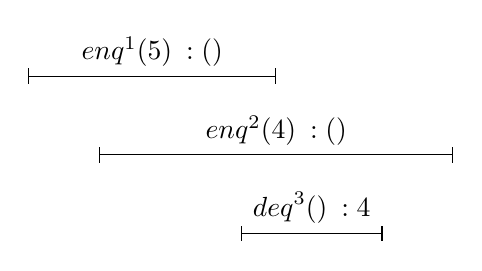
\begin{tikzpicture}[xscale = 0.9]
\draw[|-|] (0,0) -- node[above] {$\sm{enq}^1(5)\::()$} (3.5,0);
\draw (2.5,0) \X;
\draw[|-|] (1,-1) -- node[above] {$\sm{enq}^2(4)\::()$} (6,-1);
\draw (2,-1) \X;
\draw[|-|] (3,-2) -- node[above] {$\sm{deq}^3()\::4$} (5,-2);
\draw (4,-2) \X;
\end{tikzpicture}
\end{center}
\caption{Timeline representing the linearisation example.  Time runs from left
  to right; each horizontal line represents an operation execution, with the
  left-hand end representing the $\call$ event, and the right-hand end
  representing the $\return$ event.}
\label{fig:lin-timeline}
\scalaMid
\end{figure}

%%%%%

Linearisation is specified with respect to a linearisation specification
object~$Spec$, with the same operations (and signatures) as the concurrent
datatype in question.  A history of the specification object is a sequence of
events of the form:
%
\begin{itemize}
\item $op^i(x)\::y$ representing an execution of operation~$op$ with
  parameter~$x$, returning result~$y$; again $i$~is an execution identity,
  which must appear at most once in the history.
\end{itemize}
%
A history is \emph{legal} if it is consistent with the definition of~$Spec$,
i.e.~for each operation execution, the precondition is satisfied, and the
return value is as for the definition of the operation in~$Spec$.  In general,
the specification object could be nondeterministic, and so allow several
values that could be returned by an operation execution (although in all our
examples it will be deterministic).

%% We assume that the
%% specification object is deterministic: after a particular history, there is a
%% unique value that can be returned by each execution.

For example, consider the history
\begin{eqnarray*}
h_s & = & \seq{\sm{enq}^2(4)\::(),\; \sm{enq}^1(5)\::(),\; \sm{deq}^3()\::4}.
\end{eqnarray*}
%
This is a legal history for a specification object that represents a queue.
This history is illustrated by the ``$\cross$''s in
Figure~\ref{fig:lin-timeline}.

Let $h$ be a complete concurrent history, and let $h_s$ be a legal history of
the specification object~$Spec$.  We say that $h$ and~$h_s$ \emph{correspond}
if they contain the same executions, i.e., for each $\call.op^i(x)$ and
$\return.op^i\::y$ in $h$,\, $h_s$ contains $op^i(x)\::y$, and vice versa.  We
say that $h_s$ is a \emph{linearisation} of~$h$ if there is some way of
interleaving the two histories (i.e.~creating a history containing the events
of~$h$ and~$h_s$, preserving the order of events) such that each $op^i(x)\::y$
occurs between $\call.op^i(x)$ and $\return.op^i\::y$.  Informally, this
indicates that the executions of~$h$ appeared to take place in the order
described by~$h_s$, and that this order is legal according to the
specification object.  We say that $h$ is \emph{linearisable} with respect
to~$Spec$ in this case.

Continuing the running example, $h_s$ is a linearisation of~$h$, as evidenced
by the interleaving
\[
\seq{\begin{align}
  \call.\sm{enq}^1(5),\; \call.\sm{enq}^2(4),\; 
  \sm{enq}^2(4)\::(),\; \sm{enq}^1(5)\::(),\;   \call.\sm{deq}^3(), \\
  \return.\sm{enq}^1\::(),\; \sm{deq}^3\::4,\; 
  \return.\sm{deq}^3\::4,\; \return.\sm{enq}^2\::() },
  \end{align}
\]
as illustrated in  Figure~\ref{fig:lin-timeline}.
The points at which the events of~$h_s$ are inserted into~$h$ can be thought
of as the points where each operation has an effect; we refer to these as
\emph{linearisation points}. 

A concurrent history might not be complete, i.e.~it might have some pending
executions that have been called but have not returned.  An \emph{extension}
of a history~$h$ is formed by adding zero or more $\return$ events
corresponding to pending executions.  We write $complete(h)$ for the
subsequence of~$h$ formed by removing all $\call$ events corresponding to
pending executions.

We say that a (not necessarily complete) concurrent history~$h$ is
\emph{linearisable} with respect to specification object~$Spec$ if there is an
extension~$h'$ of~$h$ such that $complete(h')$ is linearisable with respect
to~$Spec$.  Informally, the $\return$ events that are in~$h'$ but not~$h$ are
for operation executions that have had an effect, but not returned in~$h$; the
$\call$ events removed in $complete(h')$ are for operation executions that
have not yet had an effect.

We say that a concurrent datatype is linearisable with respect to~$Spec$ if
each of its histories is linearisable with respect to~$Spec$.

%%%%%%%%%%%%%%%%%%%%%%%%%%%%%%%%%%%%%%%%%%%%%%%%%%%%%%%%%%%%

\subsection{Synchronisation linearisation}
\label{sec:sync-lin}

We now adapt the definition of linearisation to synchronisations.  With
standard linearisation, operations appear to take place in a one-at-a-time
order, each between the time at which the operation is invoked and when it
returns.  With synchronisation linearisation, synchronisations appear to take
place in a one-at-a-time order, with each synchronisation between the time
that each of the operations is invoked and when it returns.  In each case,
the order is one that satisfies the requirements captured by the specification
object.  

For the moment, we consider only binary heterogeneous synchronisations; we
generalise in the next section.  We consider a synchronisation object~$Sync$
with two operations, $\op_1$ and~$\op_2$, as described earlier.  A concurrent
history of~$Sync$ contains $\call$ and $\return$ events, as in the previous
subsection, corresponding to the operations~$\op_1$ and~$\op_2$.

For example, the following is a complete history of the synchronous channel
from earlier, and is illustrated in Figure~\ref{fig:sync-timeline}:
\begin{eqnarray*}
h & = & 
\seq{\begin{align}
  \call.\sm{send}^1(8),\; \call.\sm{send}^2(8),\; \call.\sm{receive}^3(()),\;
  \return.\sm{receive}^3\::8,\; \\
  \call.\sm{receive}^4(()),\; \return.\sm{send}^1\::(),\;
  \call.\sm{send}^5(9),\; \return.\sm{receive}^4\::9,\; \\
  \call.\sm{receive}^6(()),\; \return.\sm{send}^2\::(), \;
  \return.\sm{send}^5\::(),\; \return.\sm{receive}^6\::8 } .
  \end{align}
\end{eqnarray*}

%%%%%

\begin{figure}
\unScalaMid
\begin{center}
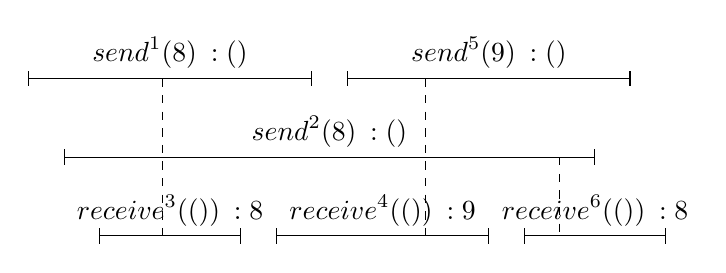
\begin{tikzpicture}[xscale = 0.9]
\draw[|-|] (0,0) -- node[above] {$\sm{send}^1(8)\::()$} (4,0);
\draw[|-|] (4.5,0) -- node[above] {$\sm{send}^5(9)\::()$} (8.5,0);
\draw[|-|] (0.5,-1) -- node[above] {$\sm{send}^2(8)\::()$} (8,-1);
\draw[|-|] (1,-2) -- node[above] {$\sm{receive}^3(())\::8$} (3,-2);
\draw[|-|] (3.5,-2) -- node[above] {$\sm{receive}^4(())\::9$} (6.5,-2);
\draw[|-|] (7,-2) -- node[above] {$\sm{receive}^6(())\::8$} (9,-2);
\draw (1.9,0) \X; \draw (1.9,-2) \X; 
\draw[dashed] (1.9,0) -- (1.9,-2); % sync 1 and 3
\draw (5.6,0) \X; \draw (5.6,-2) \X; 
\draw[dashed] (5.6,0) -- (5.6,-2); % sync 4 and 5
\draw (7.5,-1) \X; \draw (7.5,-2) \X; 
\draw[dashed] (7.5,-1) -- (7.5,-2); % sync 2 and 6 
\end{tikzpicture}
\end{center}
\caption{Timeline representing the synchronisation example.}
\label{fig:sync-timeline}
\scalaMid
\end{figure}


A history of a synchronisation specification object $Spec$ is a sequence of
events of the form $\sync^{i_1, i_2}(x_1, x_2)\:: (y_1, y_2)$, representing an
execution of |sync| with parameters $(x_1, x_2)$ and result $(y_1,y_2)$.  The
event's  identity is~$(i_1,i_2)$: each of~$i_1$ and~$i_2$ must
appear at most once in the history.  Informally, an event $\sync^{i_1,
  i_2}(x_1, x_2)\:: (y_1, y_2)$ corresponds to a synchronisation between
executions $\op_1^{i_1}(x_1)\::y_1$ and $\op_2^{i_2}(x_2)\::y_2$ in a history
of the corresponding synchronisation object.

A history is \emph{legal} if is consistent with the definition of the
specification object.
%
For example, the following is a legal history of |SyncChanSpec|.
\begin{eqnarray*}
h_s & = & 
\seq{
 \sm{sync}^{1,3}(8,()) \:: ((), 8), \;
 \sm{sync}^{5,4}(9,()) \:: ((), 9), \;
 \sm{sync}^{2,6}(8,()) \:: ((), 8) } .
\end{eqnarray*}
The history is illustrated by the ``$\cross$''s in
Figure~\ref{fig:sync-timeline}: each event corresponds to the synchronisation
of two operations, so is depicted by two ``$\cross$''s on the corresponding
operations, linked by a dashed vertical line.  
%
This particular synchronisation specification object is stateless, so in fact
any permutation of the history~$h_s$ would also be legal (but not all such
permutations will be compatible with the history of the synchronisation
object); but the same will not be true in general of a specification object
with state.
%
The points at which the events of~$h_s$ are inserted into~$h$ can be thought
of as the points where each synchronisation takes place; we refer to these as
\emph{synchronisation points}. 

%
\begin{definition}
Let $h$ be a complete history of the synchronisation object~$Sync$.  We say
that a legal history~$h_s$ of~$Spec$ \emph{corresponds} to~$h$ if their
events agree; more precisely:
\begin{itemize}
\item For each  $\sync^{i_1, i_2}(x_1, x_2)\:: (y_1, y_2)$ in~$h_s$,\,
  $h$ contains events $\call.\op_1^{i_1}(x_1)$,\,
  $\return.\op_1^{i_1}\::y_1$\,, $\call.\op_2^{i_2}(x_2)$, and
  $\return.\op_2^{i_2}\::y_2$.

\item For each $\call.\op_1^{i_1}(x_1)$ and $\return.\op_1^{i_1}\::y_1$
  in~$h$,\, $h_s$ contains an event $\sync^{i_1, i_2}(x_1, x_2)\:: (y_1, y_2)$
  for some~$i_2$, $x_2$, and~$y_2$.

\item For each $\call.\op_2^{i_2}(x_2)$ and $\return.\op_2^{i_2}\::y_2$
  in~$h$,\, $h_s$ contains an event $\sync^{i_1, i_2}(x_1, x_2)\:: (y_1, y_2)$
  for some~$i_1$, $x_1$, and~$y_1$.
\end{itemize}
%% %
%% \begin{itemize}
%% \item For each |sync| event with identity~$(i_1,i_2)$ in~$h_s$,\, $h$ contains
%%   an execution of~$\op_1$ with identity~$i_1$ and an execution of~$\op_2$ with
%%   identity~$i_2$;

%% \item For each execution of~$\op_1$ with identity~$i_1$ in~$h$,\, $h_s$
%%   contains a |sync| event with identity~$(i_1,i_2)$ for some~$i_2$;

%% \item For each execution of~$\op_2$ with identity~$i_2$ in~$h$,\, $h_s$
%%   contains a |sync| event with identity~$(i_1,i_2)$ for some~$i_1$.
%% \end{itemize}
\end{definition}

\begin{definition}
Given a complete history $h$ of~$Sync$ and a corresponding legal history $h_s$
of~$Spec$, we say that $h_s$ is a \emph{synchronisation linearisation} of~$h$
if there is some way of interleaving $h$ and~$h_s$ such that each event
$\sync^{i_1, i_2}(x_1, x_2)\:: (y_1, y_2)$ occurs between
$\call.\op_1^{i_1}(x_1)$ and $\return.\op_1^{i_1}\::y_1$, and between
$\call.\op_2^{i_2}(x_2)$ and $\return.\op_2^{i_2}\::y_2$.
\end{definition}
%
%% We say that $h$ is \emph{synchronisation-linearisable} with respect to~$Spec$
%% in this case.  
In~the running example, $h_s$ is a synchronisation
linearisation of~$h$, as shown by the interleaving in
Figure~\ref{fig:sync-timeline}.

\begin{definition}
\label{def:sync-lin-objects}
Given a (not necessarily complete) concurrent history~$h$ and a corresponding
legal history~$h_s$ of $Spec$, we say that $h_s$ is a \emph{synchronisation
  linearisation} of~$h$ if there is an extension~$h'$ of~$h$ such that $h_s$
is a synchronisation linearisation of $complete(h')$.
%
We say that $h$ is synchronisation-linearisable with respect to~$Spec$ in this
case.  We say that a synchronisation object is synchronisation-linearisable
with respect to~$Spec$ if each of its histories is
synchronisation-linearisable with respect to~$Spec$.
\end{definition}

Informally, the $\return$ events that are
in~$h'$ but not~$h$ are for operation executions that have synchronised, but
not returned in~$h$; the $\call$ events removed in $complete(h')$ are for
operation executions that have not yet synchronised.


 % formal definition of synchronisation linearisation
\section{Relating synchronisation and linearisation}

In this section we describe the relationship between synchronisation
linearisation and standard linearisation.  

\framebox{\ldots}

It is clear that synchronisation linearisation cannot, in general, be captured
directly as standard linearisation.  More precisely, given a synchronisation
linearisability specification object $SyncSpec$, it is not, in general,
possible to find a linearisability syncronisation specification $Spec$ such
that for every history~$h$,\, $h$ is synchronisation linearisable with respect
to $SyncSpec$ if and only if $h$ is linearisable with respect to $Spec$.

For example, consider the example of a synchronous channel from
Section~\ref{sec:spec}, where synchronisation linearisation is captured by
|SyncChanSpec|.  Assume (for a contradiction) that the same property can be
captured by linerisation with respect to linearisability specification~$Spec$.
Consider the history
\begin{eqnarray*}
h & = & \seq{ 
  \call.send^1(3), \call.receive^2(), 
  \return.send^1\::(), \return.receive^2()\::3 }.
\end{eqnarray*}
%
This is synchronisation linearisable with respect to |SyncChanSpec|.  By the
assumption, there must be a legal history~$h_s$ of~$Spec$ such that $h$
and~$h_s$ are compatible.  Without loss of generality, suppose the |send|
in~$h_s$ occurs before the~|receive|, i.e.
\begin{eqnarray*}
h_s & = & \seq{ send^1(3)\::(), receive^2()\::3 }.
\end{eqnarray*}
%
But the history
%
\begin{eqnarray*}
h' & = & \seq{ 
  \call.send^1(3), \return.send^1\::(), 
  \call.receive^2(), \return.receive^2()\::3 }
\end{eqnarray*}
%
is also compatible with respect to~$h_s$, so $h'$ is linearisable with respect
to~$Spec$.  But then the assumption would imply that $h'$ is synchronisation
linearisable with respect to~|SyncChanSpec|.  This is clearly false, because
the operations do not overlap.  Hence no such  linearisability
specification~$Spec$ exists.


%%%%%%%%%%%%%%%%%%%%%%%%%%%%%%%%%%%%%%%%%%%%%%%%%%%%%%%

\subsection{Two-step linearisability}

In the previous section, we showed that synchronisation linearisation does not
correspond directly to linearisation.  Nevertheless, we will show that
synchronisation linearisability corresponds to a small adaptation of
linearisability, but where one of the operations on the concurrent object
corresponds to \emph{two} operations of the linearisability specification
object.  We define what we mean by this, and then prove the correspondence in
the next subsection.  In the definitions below, we describe just the
differences from standard linearisation, to avoid repetition.

Given a synchronisation object with operations |op|\s1 and |op|\s2, as before,
we will consider a linearisability specification object with signature
%
\begin{scala}
object TwoStepLinSpec{
  def op£\s1£(x£\s1£: A£\s1£): Unit
  def £$\overline{\sm{op}}_1$£(): B£\s1£
  def op£\s2£(x£\s2£: A£\s2£): B£\s2£
}
\end{scala}
%
The idea is that the operation |op|\s1 on the concurrent object will be
linearised by the composition of the two operations |op|\s1 and
$\overline{\sm{op}}_1$; but operation |op|\s2 on the concurrent object will be
linearised by just the operation |op|\s2 of the specification object, as
before.  We call such an object a \emph{two-step linearisability specification
  object}. 

We define a history~$h_s$ of such a two-step specification object much as in
Section~\ref{sec:specification-linearisability}, except that for each event
$\overline{\sm{op}}_1^i()\::y$ in~$h_s$, we require that there is an
earlier event |op|$_1^i(x)\::()$ in~$h_s$ with the same invocation
identity; other than in this regard, invocation identities are not repeated
in~$h_s$.

Let $h$ be a complete concurrent history of a synchronisation object, and let
$h_s$ be a legal history of a two-step specification object corresponding to
the same invocations in the following sense:
%
\begin{itemize}
\item For every $\call.\sm{op}_1^i(x)$ and $\return.\sm{op}_1^i\::y$ in $h$,\,
  $h_s$~contains $\sm{op}_1^i(x)\::()$ and $\overline{\sm{op}}_1^i()\::y$; and
  vice versa;

\item For every $\call.\sm{op}_2^i(x)$ and $\return.\sm{op}_2^i\::y$ in $h$,\,
  $h_s$~contains $\sm{op}_2^i(x)\::y$; and vice versa.
\end{itemize}
%
We say that $h$ and $h_s$ are \emph{two-step compatible} if there is some way of
interleaving the two histories such that 
%
\begin{itemize}
\item Each $\sm{op}_1^i(x)\::()$ and $\overline{\sm{op}}_1^i()\::y$ occur
  between $\call.\sm{op}_1^i(x)$ and $\return.\sm{op}_1^i\::y$, in that
  order; 

\item Each $\sm{op}_2^i(x)\::y$ occurs between $\call.\sm{op}_2^i(x)$ and
  $\return.\sm{op}_2^i\::y$.
\end{itemize}

For example, consider a synchronous channel, with |send| corresponding
to~$op_1$, and |receive| corresponding to~$op_2$.  Then the following would be
an interleaving of two-step compatible histories of the synchronisation object
and the corresponding specification object.
\[
\seq{\begin{align} 
 \call.\sm{send}^1(3),\; \sm{send}^1(3)\::(),\; 
 \call.\sm{receive}^2(),\; \sm{receive}^2()\::3,\; \\
 \overline{\sm{send}}^1()\::(),\; \return.\sm{send}^1\::(), \;
 \return.\sm{receive}^2\::3 }.
\end{align}
\]

The definition of two-step linearisability then follows from this definition
of two-step compatability, precisely as in
Section~\ref{sec:specification-linearisability}.



%%%%%%%%%%%%%%%%%%%%%%%%%%%%%%%%%%%%%%%%%%%%%%%%%%%%%%%

\subsection{Proving the relationship}
\label{sec:twoStepLinSpec}

We now prove the relationship between synchronisation linearisation and
two-step linearisation.

Consider a synchonisation specification object |SyncSpec|.  We build a
corresponding two-step linearisation specification object~|TwoStepLinSpec|
such that synchronisation linearisation with respect to |SyncSpec| is
equivalent to two-step linearisation with respect to~|TwoStepLinSpec|.  The
definition is below: the specification's behaviour is described by the
automaton on the right.\footnote{Defining the subclasses of {\scalashape
    State} as {\scalashape case class}es allows pattern matching against such
  values.  For example, the statement {\scalashape val One(x}\s1{\scalashape )
    = state} succeeds only if {\scalashape state} has type {\scalashape One},
  and binds the name {\scalashape x}\s1 to the value of the {\scalashape x}\s1
  field of {\scalashape state}.}
\begin{trivlist}
\item[]
\begin{minipage}[b]{68mm}
\begin{scala}
trait State
case class Zero extends State
case class One(x£\s1£: A£\s1£) extends State
case class Two(y£\s1£: B£\s1£) extends State
\end{scala}
\end{minipage}
%
\hfil
%
\begin{minipage}[b]{63mm}
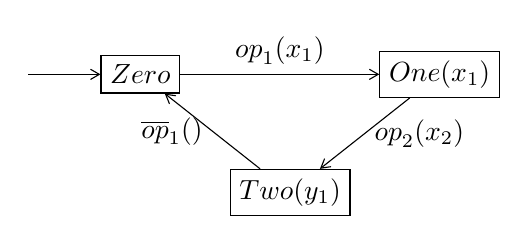
\begin{tikzpicture}[>= angle 60, xscale = 0.95, yscale = 0.75]
\draw (0,0) node[draw] (zero) {$\sm{Zero}$};
\draw[->] (zero) ++ (-1.5, 0) -- (zero);
%
\draw (4,0) node[draw] (one) {$\sm{One}(\sm{x}_1)$};
\draw[->] (zero)  -- node[above] {$\sm{op}_1(\sm{x}_1)$} (one); 
%
\draw (2, -2) node[draw] (two) {$\sm{Two}(\sm{y}_1)$};
\draw[->] (one)  -- node[right] {$\sm{op}_2(\sm{x}_2)$} (two); 
\draw[->] (two) -- node[left] {$\overline{\sm{op}}_1()$} (zero);
\end{tikzpicture}
\end{minipage}
%
%The specification object is defined as follows.
%
%% trait LinState
%% case class Zero extends LinState
%% case class One(x£\s1£: A£\s1£) extends LinState
%% case class Two(y£\s1£: B£\s1£) extends LinState
%
\begin{scala}
object TwoStepLinSpec{
  private var state: State = Zero
  def op£\s1£(x£\s1£: A£\s1£): Unit = {
    require(state.isInstanceOf[Zero]); state = One(x£\s1£)
  }
  def op£\s2£(x£\s2£: A£\s2£): B£\s2£ = {
    require(state.isInstanceOf[One]); val One(x£\s1£) = state
    val (y£\s1£, y£\s2£) = SyncSpec.sync(x£\s1£, x£\s2£); state = Two(y£\s1£); y£\s2£
  }
  def £$\overline{\sm{op}}_1$£(): B£\s1£ = {
    require(state.isInstanceOf[Two]); val Two(y£\s1£) = state; state = Zero; y£\s1£
  }
}
\end{scala}
\end{trivlist}
%
%
The definition forces the operations to take place in the order described by
the automaton.  In addition, the |op|\s2 operation calls the |sync| method on
|SyncSpec|, to calculate the return values and to update |SyncSpec|'s state;
it stores |op|\s1's result in the state. 

% in effect, the synchronisation happens at this point.

The following lemma follows immediately from the construction
of~|Two|\-|Step|\-|LinSpec|. 
%
\begin{lemma}
\label{lem:TwoStepLinSpec-histories}
Each history of~|TwoStepLinSpec| is the concatenation of triples of events of
the form $\sm{op}_1^{i_1}(x_1) \:: ()$,\, $\sm{op}_2^{i_2}(x_2) \:: y_2$,\,
$\overline{\sm{op}}_1^{i_1}() \:: y_1$ such that |SyncSpec| has a
corresponding legal history of events $\sm{sync}^{i_1,i_2}(x_1,x_2) \::
(y_1,y_2)$, and vice versa.
\end{lemma}

%%%%%

The following proposition reduces synchronisation linearisability to two-step
linearisability.
%
\begin{prop}
Let |SyncObj| be a synchronisation object, |SyncSpec| be a synchronisation
specification object, and let |TwoStepLinSpec| be built from |SyncSpec| as
above.  Then |SyncObj| is two-step linearisable with respect to
|Two|\-|Step|\-|LinSpec| if and only if it is synchronisation linearisable
with respect to |SyncSpec|.
\end{prop}
%%%%%%
\begin{proof}
\textbf{($\implies$).}\quad
%
Let $h$ be a concurrent history of |SyncObj|.  By assumption, there is an
extension $h'$ of~$h$, and a legal history~$h_s$ of |TwoStepLinSpec| such that
$h'' = complete(h')$ and~$h_s$ are two-step compatible.
%
Build a history~$h_s'$ of |SyncSpec| by replacing each triple
$\sm{op}_1^{i_1}(x_1) \:: ()$,\, $\sm{op}_2^{i_2}(x_2) \:: y_2$,\,
$\overline{\sm{op}}_1^{i_1}() \:: y_1$ in~$h_s$ by the event
$\sm{sync}^{i_1,i_2}(x_1,x_2) \:: (y_1,y_2)$.  
%
The history~$h_s'$ is legal by Lemma~\ref{lem:TwoStepLinSpec-histories}.  
%
It is possible to interleave $h''$ and~$h_s'$ by placing each event
$\sm{sync}^{i_1,i_2}(x_1,x_2) \:: (y_1,y_2)$ in the same place as the
corresponding event $\sm{op}_2^{i_2}(x_2) \:: y_2$ in the interleaving
of~$h''$ and~$h_s$; by construction, this is between
$\call.\sm{op}_1^{i_1}(x_1)$ and~$\return.\sm{op}_1^{i_1} \:: y_1$, and
between $\call.\sm{op}_2^{i_2}(x_2)$ and~$\return.\sm{op}_2^{i_2} \:: y_2$.
%
Hence $h''$ and~$h_s$ are synchronisation compatible, so $h''$ is
synchronisation lineariable, and so $h$ is synchronisation linearisable.

%%%%%

\textbf{($\Leftarrow$).}\quad
%
Let $h$ be a complete history of |SyncObj|.  By assumption, there is an
extension $h'$ of~$h$, and a legal history~$h_s$ of |SyncSpec| such that $h''
= complete(h')$ and~$h_s$ are synchronisation compatible.
%
Build a history~$h_s'$ of |TwoStepLinSpec| by replacing each event
$\sm{sync}^{i_1,i_2}(x_1,x_2) \:: (y_1,y_2)$ in~$h_s$ by the three events
$\sm{op}_1^{i_1}(x_1) \:: ()$,\, $\sm{op}_2^{i_2}(x_2) \:: y_2$,\,
$\overline{\sm{op}}_1^{i_1}() \:: y_1$.
%
The history~$h_s'$ is legal by Lemma~\ref{lem:TwoStepLinSpec-histories}.
%
It is possible to interleave $h''$ and~$h_s'$ by placing each triple
$\sm{op}_1^{i_1}(x_1) \:: ()$,\, $\sm{op}_2^{i_2}(x_2) \:: y_2$,\,
$\overline{\sm{op}}_1^{i_1}() \:: y_1$ in the same place as the corresponding
event $\sm{sync}^{i_1,i_2}(x_1,x_2) \:: (y_1,y_2)$ in the interleaving
of~$h''$ and~$h_s$; by construction, each $\sm{op}_1^{i_1}(x_1) \:: ()$ and
$\overline{\sm{op}}_1^{i_1}() \:: y_1$ are between
$\call.\sm{op}_1^{i_1}(x_1)$ and~$\return.\sm{op}_1^{i_1} \:: y_1$; and each
$\sm{op}_2^{i_2}(x_2) \:: y_2$ is between $\call.\sm{op}_2^{i_2}(x_2)$
and~$\return.\sm{op}_2^{i_2} \:: y_2$.
%
Hence $h''$ and~$h_s$ are two-step compatible, so $h''$ is two-step
lineariable, and so $h$ is two-step linearisable.
\end{proof}

%%%%%%%%%%

The two-step linearisation specification object can often be significantly
simplified from the template definition above.  Here is such a specification
object for a synchronous channel.
%
\begin{scala}
object SyncChanTwoStepLinSpec{
  private var state = 0        // Takes values 0, 1, 2, cyclically 
  private var value: A = _    // The current value being sent
  def send(x: A): Unit = { require(state == 0); value = x; state = 1 }
  def receive(u: Unit): A = { require(state == 1); state = 2; value }
  def £$\overline{\sm{send}}$£(): Unit = { require(state == 2); state = 0 }
}
\end{scala}
 % relating synchronisation linearisation and linearisation
\section{Linearisability testing}
\label{sec:lin-testing}

In the following two sections, we describe techniques for testing whether the
implementation of a synchronisation object is synchronisation linearisable
with respect to a synchronisation specification object.
%
The techniques are influenced by the techniques for testing (standard)
linearisation~\cite{wing-gong,gavin:lin-testing}, so we begin by sketching
those techniques.

The idea of linearisability testing is as follows.  We run several
\emph{worker threads}, performing operations (typically chosen randomly) upon
the concurrent datatype that we are testing, and logging the calls and
returns.  More precisely, a thread that performs a particular
operation~$\sm{op}^i(x)$: (1) writes $\call.\sm{op}^i(x)$ into the log;
(2)~performs $\sm{op}(x)$ on the synchonisation object, obtaining result~$y$,
say; (3)~writes $\return.\sm{op}^i \:: y$ into the log.  Further, the logging
associates each operation execution with an execution $\sm{op}(x)$ of the
corresponding operation on the specification object.

Once all worker threads have finished, we can use an algorithm to test whether
the history is linearisable with respect to the specification object.  The
algorithm searches for an order to linearise the executions, consistent with
the log, and such that the order represents a legal history of the
corresponding executions on the specification object.
See~\cite{wing-gong,gavin:lin-testing} for details of several algorithms.
All these algorithms assume that the specification object is deterministic.

This process can be repeated many times, so as to generate and analyse many
histories.  Our experience is that the technique works well.  It seems
effective at finding bugs, where they exist, typically within a few seconds;
for example, we used it to find an error in the concurrent priority queue
of~\cite{faulty-pri-queue}, which we believe had not previously been
documented.  Further, the technique is easy to use: we have taught it to
undergraduate students, who have used it effectively.

This testing concentrates upon the safety property of
linearisation, rather than liveness properties such as deadlock-freedom.
However, if the concurrent object can deadlock, it is likely that the testing
will discover this.  Related to this point, it is the responsibility of the
tester to define the worker threads in a way that all executions will
eventually return, so the threads terminate.  For example, consider a partial
stack where a |pop| operation blocks while the stack is empty; here, the
tester would need to ensure that threads collectively perform at least as many
|push|es as |pop|s, to ensure that each |pop| does eventually return.

Note also that there is potentially a delay between a worker thread writing the
$\call$ event into the log and actually calling the operation; and likewise
there is potentially a delay between the operation returning and the thread
writing the $\return$ event into the log.  However, these delays do not
generate false errors: if a history without such delays is linearisable, then
so is a corresponding history with delays.  We believe that it is essential
that the technique does not give false errors: an error reported by testing
should represent a real error; testing of a correct implementation should be
able to run unsupervised, maybe for a long time.  Further, our experience is
that the delays do not prevent the detection of bugs when they exist (although
might require performing the test more times).  This means that a failure to
find any bugs, after a large number of tests, can give us good confidence in
the correctness of the concurrent datatype.

%%%%%%%%%%%%%%%%%%%%%%%%%%%%%%%%%%%%%%%%%%%%%%%%%%%%%%%

\section{Adapting the linearisability framework}
\label{sec:testing-hacking}

In this section we investigate how to use the existing linearisation testing
framework for testing synchronisation linearisation, using the ideas of
Section~\ref{sec:relating}.  We require the synchronisation specification
object to be deterministic, reflecting the fact that the linearisation
testing framework requires its specification object to be deterministic.  

This is not a use for which the framework was intended, so we consider it a
hack.  However, it has the advantage of not requiring the implementation of
any new algorithms.  (We do not consider progressibility in this section.)

%% Recall, from the introduction of Section~\ref{sec:relating}, that a
%% straightforward approach won't work.  Instead 

We adapt the idea of two-step linearisation from Section~\ref{sec:relating}.
We start by considering the case of binary heterogeneous synchronisation.  We
aim to obtain a log history that can be tested for (standard) linearisation
against |TwoStepLinSpec|.

As with standard linearisability testing, we run several worker threads,
calling operations on the synchronisation object, and logging the calls and
returns.
%
\begin{itemize}
\item A thread~$t_1$ that performs the concrete operation~$\op_1(x_1)$:
  (1)~writes $\call.\sm{op}_1^{i_1}(x_1)$ into the log, associating it with a
  corresponding execution $\op_1(t_1, x_1)$ on the specification object;
  (2)~performs $\op_1(x_1)$ on the synchonisation object, obtaining
  result~$y_1$, say; (3)~writes $\return.\op_1^{i_1} \:: ()$ into the log;
  (4)~writes $\call.\overline{\op}_1^{i_1}()$ into the log, associating it
  with a corresponding execution $\overline{\op}_1(t)$ on the specification
  object; (5)~writes $\return.\overline{\op}_1^{i_1} \:: y_1$ into the log.

\item A thread~$t_2$ that performs operation~|op|\s2, acts as for standard
  linearisability testing.  It: (1)~writes $\call.\sm{op}_2^{i_2}(x_2)$ into
  the log, associating it with a corresponding execution $\op_2(x_2)$ on the
  specification object; (2)~performs $\op_2(x_2)$ on the synchonisation
  object, obtaining result~$y_2$, say; (3)~writes $\return.\op_2^{i_2} \::
  y_2$ into the log
\end{itemize}
%
The top half of Figure~\ref{fig:twostep-timeline} illustrates a possible run,
containing a single synchronisation, together with the log history.

\begin{figure}
\begin{center}
\def\y{-1.4} % op_2 y-coord
\def\ySLin{-2.5} % sync-lin y-ccord
\def\yLin{-3.6} % linearisation y-coord
\begin{tikzpicture}%[yscale = 1.4]
\bulletAt(-0.6,0){$\call.\op_1(x_1)$};
\draw[|-|] (0.0,0) -- node[above] {$\op_1(x_1)\::y_1$} (2.5,0);
\bulletAt(3.1,0){$\return.\op_1$};
\bulletAt(4.7,0){$\call.\overline{\op}_1$};
\bulletAt(6.5,0){$\return.\overline{\op}_1\::y_1$};
%
\bulletAt(-0.3,\y){$\call.\op_2(x_2)$};
\draw[|-|] (0.4,\y) -- node[above]{$\op_2(x_2)\::y_2$} (2.7,\y);
\bulletAt(3.5,\y){$\return.\op_2\::y_2$};
%
\draw (-2,\ySLin) node{$h_s$};
\crossAt(1.4,\ySLin){$\sync(x_1,x_2)\::(y_1,y_2)$};
%
\draw (-2,\yLin) node{$h_{2s}$:};
\draw(1.2,\yLin) \X; 
\draw(0.5,\yLin-0.4) node{\footnotesize $\op_1(t_1,x_1)$};
\draw(1.6,\yLin) \X;
\draw(2.3,\yLin-0.4) node{\footnotesize $\op_2(x_2)\::y_2$};
%% \crossAt(0.5,\yLin){$\op_1(t_1,x_1)$};
%% \crossAt(2.3,\yLin){$\op_2(x_2)\::y_2$};
\crossAt(5.5,\yLin){$\overline{\op}_1(t_1)\::y_1$};
\end{tikzpicture}
\end{center}
\caption{Illustration of two-step linearisation testing.  The operation
  executions are represented by the horizontal lines with labels above
  (denoted ``$h$'' in Proposition~\ref{prop:twostep-testing}).  The log
  entries are represented by the bullets with labels below (denoted ``$h_l$''
  in Proposition~\ref{prop:twostep-testing}).  Linearisation points are
  represented by crosses with labels below: the penultimate row, labelled
  ``$h_s$'', is a synchronisation linearisation; the bottom row, labelled
  ``$h_{2s}$'', is a linearisation of the two-step synchronisation object.
  Execution identifiers and null arguments and returns are omitted, for
  clarity.}
\label{fig:twostep-timeline}
\end{figure}

%%%%%

Once all threads have finished, we test whether the log history is
linearisable (i.e.~standard linearisation) with respect to |TwoStepLinSpec|
from Section~\ref{sec:relating}.  Figure~\ref{fig:twostep-timeline} gives an
example linearisation, denoted~$h_{2s}$.

Note that we have three related concepts here: (1)~synchronisation
linearisation of the concrete history of operation executions with respect to
|SyncSpec|; (2)~two-step linearisation of the concrete history with respect
to~|TwoStepLinSpec|; and (3)~linearisation of the log history with respect
to~|TwoStepLinSpec|.  Proposition~\ref{prop:two-step-lin} shows that the first
two of these are equivalent.  We need to show that these imply~(3), so the
technique does not give false errors.  (The converse might not hold, because
of delays in writing to the log.)

Since the linearisation algorithm receives  a log history, rather
than a concrete history, we need to describe the relationship.  
%% The following definition captures that a log history~$h_l$ might arise from a
%% concrete history~$h$, using the logging strategy described above.
%
\begin{definition}
Let $h$ be a complete history of a binary heterogeneous synchronisation
object, and let $h_l$ be a log history for the same object.  We say that the
two histories \emph{correspond} if there is some way of interleaving them such
that
%
\begin{itemize}
\item Each $\call.\op_1^{i_1}(x_1)$, from $h_l$, precedes the call and return
  of~$\op_1^{i_1}(x_1)\::y_1$ from~$h$, which precede $\return.\op_1^{i_1} \::
  ()$, $\call.\overline{\op}_1^{i_1}()$ and $\return.\overline{\op}_1^{i_1}
  \:: y_1$, from~$h_l$, in that order.

\item Each $\call.\op_2^{i_2}(x_2)$, from $h_l$, precedes the call and return
  of~$\op_2^{i_2}(x_2)\::y_2$ from~$h$, which precede $\return.\op_2^{i_2}
  \:: y_2$, from~$h_l$.
\end{itemize}
\end{definition}

\begin{prop}
\label{prop:twostep-testing}
Let $h$ be a complete history of a binary heterogeneous synchronisation
object, and let $h_l$ be a corresponding log history for the same object.  Let
|SyncSpec| be a synchronisation specification object, and |TwoStepSyncSpec|
the corresponding two-step synchronisation specification object, constructed
as in Section~\ref{sec:twoStepLinSpec}.  Suppose $h$ is
synchronisation-linearisable with respect to |SyncSpec|.  Then $h_l$ is
linearisable with respect to |TwoStepSyncSpec|.
\end{prop}
%
\begin{proof}
Since $h$ is synchronisation-linearisable, there is a legal history~$h_s$ of
|SyncSpec| such that $h_s$ is a synchronisation linearisation of $h$.
Consider the interleaving of $h_s$ and~$h$, that demonstrates this, and
interleave $h_l$ with it, consistent with the interleaving of~$h$ and~$h_l$
that demonstrates that they correspond.  Figure~\ref{fig:twostep-timeline}
illustrates such an interleaving.

We build a history~$h_{2s}$ of~|TwoStepSyncSpec|, and interleave it with~$h_l$
as follows.  In the interleaving of the previous paragraph, replace each event
$\sync^{i_1,i_2}(x_1,x_2)\::(y_1,y_2)$ (from~$h_s$) by immediately consecutive
events~$\op_1^{i_1}(x_1)\::()$ and $\op_2^{i_2}(x_2)\::y_2$, and add
$\overline{\op}_1^{i_1}()\::y_1$ between $\call.\overline{\op}_1^{i_1}()$ and
$\return.\overline{\op}_1^{i_1} \:: y_1$ (from~$h_l$).  Again,
Figure~\ref{fig:twostep-timeline} illustrates such an interleaving.  This is a
legal history of~|TwoStepSyncSpec|, by
Lemma~\ref{lem:TwoStepLinSpec-histories}.  Further, each event of~$h_{2s}$ is
between the corresponding $\call$ and $\return$ events of~$h_l$, by
construction.  Hence $h_{2s}$ is a linearisation of~$h_l$.
\end{proof}

%%%%%%%%%%%%%%%%%%%%%%%%%%%%%%%%%%%%%%%%%%%%%%%%%%%%%%%

%% \subsection{OLD VERSION}

%% Note there might be delays involved in writing to the log, so that the log
%% history does not correspond precisely to the history of operation calls and
%% returns.  We show that the approximation serves our purposes.

%% Consider a history~$h$ of the synchronisation object, and suppose, for the
%% moment, there are no delays in logging, i.e.:\ (1)~the $\call.\op_1$ and
%% $\call.\op_2$ events happen immediately before the actual calls; (2)~the
%% $\return.\op_2$ events happen immediately after the return of~$\op_2$; and
%% (3)~the $\call.\overline\op_1$ and $\return.\overline\op_1$ events happen
%% immediately after the return of $\op_1$ --- in each case with no intervening
%% events.  Then the log history is linearisable with respect to |TwoStepLinSpec|
%% if and only if the history~$h$ is two-step linearisable with respect to
%% |TwoStepLinSpec|.  But Proposition~\ref{prop:two-step-lin} then shows that
%% this holds if and only if $h$ is synchronisation linearisable.  In particular,
%% this shows that errors are detected providing the logging is fast enough.

%% We now show that delays in logging do not introduce false errors.  Consider a
%% history~$h$ that is synchronisation linearisable, and consider the
%% corresponding log history~$h_l$.  Now build a history~$h'$ so that each
%% operation is extended so that: (1)~each call of~$\op_1$ or~$\op_2$ is
%% immediately before the $\call.\op_1$ or $\call.\op_2$ event in~$h_l$; (2)~each
%% return of~$\op_1$ is immediately after the $\return.\overline\op_1$ event
%% in~$h_l$; and (3)~each return of~$\op_2$ is immediately after the
%% $\return.\op_2$ event in~$h_l$.  This construction is illustrated below for
%% the two types of operation.
%% %
%% \begin{center}
%% \begin{tikzpicture}[xscale = 1.0, yscale = 1.0]
%% \draw (-2.0,0) node{$h$:};
%% \draw (-2.0,-1) node{$h_l$:};
%% \draw (-2.0,-2.3) node{$h'$:};
%% % op_1^1
%% \draw[|-|] (0,0) -- node[above] {$\sm{op}_1(x_1)\::y_1$} (1,0);
%% \bulletAt(-0.2,-0.8){$\call.\sm{op}_1$}
%% \bulletAt(1.2,-0.8){$\return.\sm{op}_1$}
%% \bulletAt(2.7,-0.8){$\call.\overline{\op}_1$}
%% \bulletAt(4.2,-0.8){$\return.\overline{\op}_1$}
%% \draw[|-|] (-0.4,-2.3) -- node[above] {$\sm{op}_1(x_1)\::y_1$} (4.4,-2.3);
%% %%%%%
%% \draw[|-|] (7.0,0) -- node[above] {$\sm{op}_2(x_2)\::y_2$} (8,0);
%% \bulletAt(6.8,-0.8){$\call.\sm{op}_2$}
%% \bulletAt(8.2,-0.8){$\return.\op_2$}
%% \draw[|-|] (6.6,-2.3) -- node[above] {$\sm{op}_2(x_2)\::y_2$} (8.4,-2.3);
%% \end{tikzpicture}
%% \end{center}
%% %
%% Now $h$ is synchronisation linearisable; and hence $h'$ is also (since each
%% operation in $h'$ is an extension of the corresponding operation in~$h$).  But
%% then Proposition~\ref{prop:two-step-lin} implies that $h'$ is two-step
%% linearisable with respect to |TwoStepLinSpec|.  Hence $h_l$ is linearisable
%% with respect to |TwoStepLinSpec|, by construction.

This approach generalises to non-binary synchronisations, homogeneous
synchronisations, and stateful specification objects as in
Section~\ref{ssec:relating-variations}.


As with standard linearisation, the tester needs to define the worker threads
so that all executions will eventually return, i.e.~so that each will be able
to synchronise.  For a binary heterogeneous synchronisation with no
precondition, we can achieve this by half the threads calling one operation,
and the other half calling the other operation (with the same number of calls
by each).  For a binary homogeneous synchronisation, this approach might not
work if every worker does more than one operation: one worker might end up
with two operations to perform, when all others have terminated; instead, we
arrange for an even number of workers to each perform a single operation.


%%%%%%%%%%%%%%%%%%%%%%%%%%%%%%%%%%%%%%%%%%%%%%%%%%%%%%%

\paragraph{Variable-arity synchronisations}

It turns out that it is not, in general, possible to capture variable-arity
synchronisations using this technique, in particular where the arity of a
synchronisation depends upon the relative timing of executions, as opposed to
the state of the specification object.  This is a result of two things: that
the logging of operations, in particular the $\overline{\op}_1$, can be
arbitrarily delayed; and that it can be nondeterministic whether or not two
executions synchronise, which is at odds with the fact that each operation on
the specification object needs to be deterministic.

To illustrate this point, consider a timeout channel.  Without loss of
generality, let the |send| operation correspond to $\op_1$, and the
|receive| operation correspond to~$\op_2$.

The top-half of Figure~\ref{fig:two-step-timeout-channel} gives a
timeline illustrating a successful |send(3)| and |receive|.  This
corresponds to the history
\[
\seq{ \send(3)\::(),\; \receive()\::\sm{Some}(3),\; 
  \overline{\send}()\::\sm{true} }
\]
of the specification object.

%%%%%%%%%%

\begin{figure}
\begin{center}
\def\yLin{-2.5} % y-coord for linearisation
\begin{tikzpicture}[xscale = 0.9]
\bulletAt(-0.4,0){$\call.\send(3)$};
\draw[|-|] (0,0) -- node[above] {$\send(3)\::()$} (1.6,0);
\bulletAt(2.0,0){$\return.\send$};
%
\bulletAt(3.9,0){$\call.\overline{\send}$};
\bulletAt(6.2,0){$\return.\overline{\send}\::\sm{true}$};
%
\bulletAt(-0.5,-1.5){$\call.\receive\qquad$};
\draw[|-|] (0.3,-1.5) -- 
  node[above] {$\receive()\::\sm{Some}(3)$} (1.9,-1.5);
\bulletAt(2.8,-1.5){\ $\qquad\qquad\return.\receive\::\sm{Some(3)}$};
%
\draw(0.7,\yLin) \X; 
\draw(-0.1,\yLin-0.4) node{\footnotesize $\send(3)\::()$};
\draw(1.1,\yLin) \X;
\draw(2.6,\yLin-0.4) node{\footnotesize $\receive()\::\sm{Some}(3)$};
%% \crossAt(0.7,-3){$\send(3)\::()$}
%% \crossAt(1.5,-3){$\receive()\::\sm{Some}(3)$}
\crossAt(5.5,\yLin){$\overline{\send}\::\sm{true}$}
%
\draw (-2.2,-3.6) -- ++(12.4,0); 
\end{tikzpicture}

%%%%%%
%\hfil\hfil
\medskip

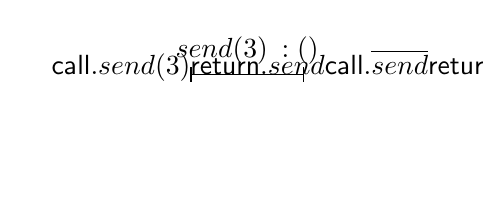
\begin{tikzpicture}[xscale = 0.9]
\bulletAt(-0.4,0){$\call.\send(3)$};
\draw[|-|] (0,0) -- node[above] {$\send(3)\::()$} (1.6,0);
\bulletAt(2.0,0){$\return.\send$};
%
\bulletAt(7.1,0){$\call.\overline{\send}$};
\bulletAt(9.4,0){$\return.\overline{\send}\::\sm{false}$};
%
\bulletAt(2.5,-1.5){$\call.\receive\qquad$};
\draw[|-|] (3.3,-1.5) -- 
  node[above] {$\receive()\::\sm{None}$} (4.9,-1.5);
\bulletAt(5.8,-1.5){\ $\qquad\qquad\return.\receive\::\sm{None}$};
%
\crossAt(0.8,\yLin){$\send(3)\::()$};
\crossAt(3.9,\yLin){$\receive()\::\sm{Some}(3)$};
\crossAt(8.2,\yLin){$\overline{\send}\::\sm{true}$}
%% \draw[|-|] (0,-3.5) -- node[above] {$\send(3)\::()$} (1.6,-3.5);
%% \crossAt(0.7,-3.5){$\send(3)\::()$}
%% %
%% \draw[|-|] (2.2,-5) -- 
%%   node[above] {$\receive()\::\sm{None}$} (3.8,-5);
%% \crossAt(3.4,-5){$\receive()\::\sm{Some}(3)$}
%% %
%% \draw[|-|] (4.0,-3.5) -- node[above] 
%%   {$\overline{\send}(3)\::\sm{false}$} (5.6,-3.5);
%% \crossAt(4.8,-3.5){$\overline{\send}(3)\::\sm{true}$}
\end{tikzpicture}
\end{center}
\caption{Figure showing why two-step linearisation cannot be used for a
  timeout channel.  Conventions are as in Figure~\ref{fig:twostep-timeline}.}
\label{fig:two-step-timeout-channel}
\end{figure}

%%%%%%%%%%

The bottom-half side of Figure~\ref{fig:two-step-timeout-channel} gives a
timeline illustrating an unsuccessful |send(3)| and |receive|, and where the
logging of $\overline{\send}$ is delayed.  None of the executions overlap, so
they must necessarily be linearised in the same order as in the previous
history.  The specification object is deterministic, so the operations must
return the same results as in the previous history.  But, in the cases of
$\receive$ and $\overline{\send}$, those returned values, |Some(3)| and
|true|, do not agree with the corresponding values in the log history, |None|
and |false|.  Hence the history would be flagged as an error, despite being
valid.

The difference between this situation and the discussion in
Section~\ref{ssec:relating-variations} is that the logging of
operations, in particular the $\overline{\send}$, can be arbitrarily delayed.
However, in the earlier section we allowed the $\overline{\send}$ anywhere
within the corresponding concrete operation.  This means that a history like
in the bottom-half of Figure~\ref{fig:two-step-timeout-channel} could be
linearised by the history
\[
\seq{ \send(3)\::(),\; \overline{\send}(3)\::\sm{false},\;
  \receive()\::\sm{None} }
\]
of the two-step specification object.  Here the operations take place in a
different order than for Figure~\ref{fig:two-step-timeout-channel}, and so
this is consistent with a deterministic specification object.

A similar problem arises with a timeout exchanger.

%\framebox{Explain how it can be done.}

We have investigated an alternative approach, which involves worker threads
adapting their logging behaviour based on the outcome of their operations.
For the timeout channel:
\begin{itemize}
\item A thread that sends a value~$x$: (1)~writes $\call.\send^{i_1}(x)$ into
  the log; (2)~performs $\send(x)$ on the channel; (3)~writes
  $\return.\send^{i_1} \:: ()$ into the log; (4)~if the send is successful,
  associates the log entries with an operation $\send(x)$ on the specification
  object, and otherwise associates them with an operation $\sm{sendFail}(x)$;
  (5)~if the send is successful, writes $\call.\overline{\send}^{i_1}()$ and
  $\return.\overline{\send}_1^{i_1} \:: ()$ into the log, associating them
  with an operation $\overline{\send}()$ on the specification object (and
  otherwise does nothing).

%%     (6)~writes $\return.\overline{\send}_1^{i_1} \:: ()$ into the log

%% then:
%%   \begin{itemize}
%%   \item if the send is successful: (4) associates the log entries with an
%%     operation $\send(x)$ on the specification object; (5)~writes
%%     $\call.\overline{\send}^{i_1}()$ into the log, associating it with a
%%     corresponding execution $\overline{\send}()$ on the specification object;
%%     (6)~writes $\return.\overline{\send}_1^{i_1} \:: ()$ into the log.

%%   \item if the send is unsuccessful: (4)~associates the log entries with an
%%     operation $\sm{sendFail(x)}$ on the specification object (and does not
%%     perform the second step).
%%   \end{itemize}

\item A thread that performs a receive: (1)~writes $\call.\receive^{i_2}$ into
  the log; (2)~performs $\receive$ on the channel, receiving result~$r$, say;
  (3)~writes $\return.\receive^{i_1} \:: r$ into the log; (4)~if the receive
  was successful, associates the log entries with an operation |receive| on
  the specification, and otherwise associates them with an
  operation $\sm{receiveFail}$.
\end{itemize}



\begin{window}[0,r,{
\begin{minipage}{48.5mm}
\begin{tikzpicture}[>= angle 60]
\draw (0,0) node[draw] (zero) {$\sm{Zero}$};
\draw[<-] (zero) -- ++ (-1.5,0);
\loopRight(zero){$
%% \draw[->] (zero) .. controls ++(1.5,0.4) and (1.5,-0.4) .. node[right] {$
  \begin{align} 
  \sm{sendFail}, \\ \overline{\send}, \\ \sm{receiveFail}
  \end{align}$}% (zero);
%
\draw (0,-2) node[draw] (one) {$\sm{One}(\sm{x})$};
\draw[->] (zero) .. controls ++(0.3,-1) .. node[right] {$\sm{send(x)}$} (one); 
\draw[->] (one) .. controls ++(-0.3,1) .. 
  node[left] {$\begin{align}\sm{receive}\::\\ \quad\sm{Some(x)}\end{align}$} (zero);
\end{tikzpicture}
\end{minipage}
},] 
The specification object then encodes the automaton to the right.
Thus a successful synchronisation is linearised by the sequence $\send(\sm x)$,
$\receive\::\sm{Some(x)}$, $\overline{\send}$, with the former two events
consecutive, as for other binary heterogeneous synchronisations.  Unsuccessful
sends and receives are each linearised by a single event.
\end{window}

%%%%%%%%%%%%%%%%%%%%%%%%%%%%%%%%%%%%%%%%%%%%%%%%%%%%%%%

%% The specification object then encodes the automaton below. 
%% %% \begin{window}[0,r,{
%% %% \begin{minipage}{73mm}
%% \begin{center}
%% \begin{tikzpicture}[>= angle 60]
%% \draw (0,0) node[draw] (zero) {$\sm{Zero}$};
%% \draw[<-] (zero) -- ++ (-1.5,0);
%% \loopAbove(zero){$
%% %% \draw[->] (zero) .. controls ++(1.5,0.4) and (1.5,-0.4) .. node[right] {$
%%   \begin{array}{c} 
%%   \sm{sendFail}, \overline{\send}, \\ \sm{receiveFail}
%%   \end{array}$}% (zero);
%% %
%% \draw (4,0) node[draw] (one) {$\sm{One}(\sm{x})$};
%% \draw[->] (zero) .. controls ++(2,0.3) .. node[above] {$\sm{send(x)}$} (one); 
%% \draw[->] (one) .. controls ++(-2,-0.3) .. 
%%   node[below] {$\sm{receive}\::\sm{Some(x)}$} (zero);
%% \end{tikzpicture}
%% \end{center}
%% %% \end{minipage}
%% %% },] 
%% Thus a successful synchronisation is linearised by the sequence $\send(\sm x)$,
%% $\receive\::\sm{Some(x)}$, $\overline{\send}$, with the former two events
%% consecutive, as for other binary heterogeneous synchronisations.  Unsuccessful
%% sends and receives are each linearised by a single event.

A similar technique can be used for a timeout exchanger.  We consider this
approach convoluted, and we do not advocate it.  We include it only for
completeness.

 % testing algorithms
\section{Direct testing of synchronisation linearisation}
\label{sec:direct}

We now consider how to test for synchronisation linearisation more directly.
We perform logging precisely as for standard linearisation: a thread that
performs a particular operation~$\sm{op}^i(x)$: (1) writes
$\call.\sm{op}^i(x)$ into the log; (2)~performs $\sm{op}(x)$ on the
synchonisation object, obtaining result~$y$, say; (3)~writes
$\return.\sm{op}^i \:: y$ into the log.

In this section we consider algorithms for determining if the resulting log
history is synchronisation linearisable.  In Section~\ref{sec:algorithm-dfs}
we present a general algorithm for this problem, based on depth-first search.
We then consider the complexity of this problem.  We show, in
Section~\ref{sec:NP-complete}, that the problem of deciding whether a history
is synchronisation linearisable is NP-complete in general.  Nevertheless, we
show that in the case of binary synchronisations with a stateless
specification object the problem can be solved in polynomial time: we consider
the heterogeneous case in Section~\ref{sec:binary-heterogeneous}, and the
homogeneous case in Section~\ref{sec:binary-homogeneous}.  However, in
Section~\ref{sec:non-binary-stateless} we show that for synchronisations of
three or more invocations, the problem is again NP-complete, even in the
stateless case.

%%  It turns out that the appropriate
%% algorithm, and corresponding complexity results, differ depending upon the
%% nature of the synchronisation object: whether synchronisations are binary, or
%% may involve more than two threads; and whether the object is stateful or
%% stateless. 

%% Main ideas: general algorithm; NP-complete in general case; quadratic in
%% stateless binary heterogeneous case; polynomial in binary homogeneous case;
%% NP-complete for synchronisations of arity more than~2 even in stateless case


%%%%%%%%%%%%%%%%%%%%%%%%%%%%%%%%%%%%%%%%%%%%%%%%%%%%%%%%%%%%

\subsection{The general case}
\label{sec:algorithm-dfs}

We describe an algorithm for deciding whether a given complete history~$h$ is
synchronisation linearisable with respect to a given synchronisation
specification object.  We transform the problem into a graph-search algorithm
as follows.

We define a search graph, where each node is a \emph{configuration}
comprising:
%
\begin{itemize}
\item An index $i$ into the log;

\item A set $pending$ of operation invocations that were called in the
  first~$i$ events of the log and that have not yet been linearised;

\item A set $linearised$ of operation invocations that were called in the
  first~$i$ events of the log and that have been linearised, but have not yet
  returned;

\item The state $spec$ of the specification object after the synchronisations
  linearised so far.
\end{itemize}
%
From such a configuration, there are edges to configurations as follows:
%
\begin{description}
\item[Synchronisation.] If some set of invocations in $pending$ can
  synchronise, giving results compatible with~$spec$, then there is an edge to
  a configuration where the synchronising invocations are moved into
  $linearised$, and the specification object is updated corresponding to the
  synchronisation;

\item[Call.] If the next event in the log is a $\call$ event, then there is an
  edge where that event is added to $pending$, and $i$ is advanced;

\item[Return.] If the next event in the log is a $\return$ event, and the
  corresponding invocation is in $linearised$, then that invocation is removed
  from $linearised$, and $i$ is advanced.
\end{description}
%
The initial configuration has $i$ at the start of the log, $pending$ and
$linearised$ empty, and $spec$ the initial state of the specification object.
Target configurations have $i$ at the end of the log, and $pending$ and
$linearised$ empty.  

Any path from the initial configuration to a target configuration clearly
represents an interleaving of a history of the specification object with~$h$,
as required for compatibility.  We can therefore search this graph using a
standard algorithm.  Our implementation uses depth-first search.

\framebox{**} Our implementation employs a partial-order reduction.  This
allows synchronisation edges only after a call edge or another synchronisation
edge, with the first synchronisation in each such sequence including the
invocation corresponding to the call.  \framebox{**} Test whether this
actually helps.  If so, justify better.


%% Suppose the specification object has non-trivial state. 

%% I think it will be more efficient to give a more direct implementation.
%% Define a configuration to be: (1)~a point in the log reached so far; (2)~the
%% set of pending operation invocations that have not synchronised; (3)~the set
%% of pending operation invocations that have synchronised (but not returned);
%% and (4)~the state of the sequential synchronisation object.  In any
%% configuration, can: synchronise a pair of pending operations (and update the
%% synchronisation object); advance in the log if the next event is a return that
%% is not pending; or advance in the log if the next event is a call.  Then
%% perform DFS.

%% Partial order reduction: a synchronisation point must follow either the
%% call of one of the concurrent operations, or another synchronisation
%% point.  Any synchronisation history can be transformed into this form, by
%% moving synchronisation points earlier, but not before any of the corresponding
%% call events, and preserving the order of synchronisations.  This means that
%% after advancing past the call of an invocation, we may synchronise that
%% invocation, and then an arbitrary sequence of other invocations. 

%% Alternatively, a synchronisation point must precede either the return of one
%% of the concurrent operations, or another synchronisation point.  This is more
%% like the JIT technique in the linearisability testing paper.  This means that
%% before advancing in the log to the return of an invocation that has not
%% synchronised, we synchronise some invocations, ending with the one in
%% question.  And we only synchronise in these circumstances. 

%% My intuition is that the former is more efficient: in the latter, we might
%% investigate synchronising other invocations even though the returning
%% operation can't be synchronised with any invocation.  

%%%%%%%%%%%%%%%%%%%%%%%%%%%%%%%%%%%%%%%%%%%%%%%%%%%%%%%

\subsection{Complexity}
\label{sec:NP-complete}

Consider the problem of testing whether a given concurrent history is
synchronisation linearisable with respect to a given synchronisation
specification object.  We show that this problem is NP-complete in general.


%%  It is clearly in NP: a
%% suitable certificate would be the interleaving with the corresponding history
%% of the specification object.

We make use of a result from~\cite{???} concerning the complexity of the
corresponding problem for linearisability.  Let |Variable| be a
linearisability specification object corresponding to a variable with |get|
and |set| operations.  Then the problem of deciding whether a given concurrent
history is linearisable with respect to |Variable| is NP-complete.

Since standard linearisation is a special case of synchronisation
linearisation (in the trivial case of no synchronisations), this immediately
implies that deciding synchronisation linearisation is NP-complete.  However,
even if we restrict to the non-trivial case of binary synchronisations, the
result still holds.

We consider concurrent synchronisation histories on an object with the
following signature, which mimics the behaviour of a variable but via
synchronisations. 
%
\begin{scala}
object VariableSync{
  def op£\s1£(op: String, x: Int): Int
  def op£\s2£(u: Unit): Unit
} 
\end{scala}
%
The intention is that |op|\s1|("get", x)| acts like |get(x)|, and
|op|\s1|("set", x)| acts like |set(x)| (but returns -1).  The |op|\s2
invocations do nothing except synchronise with invocations of~|op|\s1.  This
can be captured formally by the following synchronisation specification
object.
%
\begin{scala}
object VariableSyncSpec{
  private var state = 0
  def sync((op, x): (String, Int), u: Unit): (Int, Unit) = 
    if(op == "get") (state, ()) else{ state = x; (-1, ()) }
}
\end{scala}


Let |ConcVariable| be a concurrent object that represents a variable.  Given a
history~$h$ of |ConcVariable|, we build a history~$h'$
of |VariableSync| as follows.  We replace every call or return of |get(x)| by
(respectively) a call or return of |op|\s1|("get", x)|; and we do similarly
with |set|s.  If there are $k$ calls of |get| or |set| in total, we prepend
$k$ calls of |op|\s2, and append $k$ corresponding returns (in any order).
%
Then it is clear that $h$ is linearisable with respect to |Variable| if and
only if $h'$ is linearisable with respect to |VariableSyncSpec|.  Deciding the
former is NP-complete; hence the latter is also. 



%%%%%%%%%%%%%%%%%%%%%%%%%%%%%%%%%%%%%%%%%%%%%%%%%%%%%%%

\subsection{The binary heterogeneous stateless case}
\label{sec:binary-heterogeneous}

The result of the previous subsection used a stateful specification object.
We now consider the stateless case for binary heterogeneous synchronisations.
We show that in this case the problem of deciding whether a history is
synchronisation linearisable can be decided in quadratic time.

So consider a binary synchronisation object, whose specification object is
stateless.  Note that in this case we do not need to worry about the order of
synchronisations: if each individual synchronisation is correct, then any
permutation of them will be synchronisation-linearisable.

Define two invocations to be \emph{compatible} if they could be synchronised,
i.e.~they overlap and the return values agree with those for the specification
object.  For $n$ invocations of each operation (so a history of length~$4n$),
this can be calculated in $O(n^2)$.

Consider the bipartite graph where the two sets of nodes are invocations
of~$\op_1$ and~$\op_2$, respectively, and there is an edge between two
invocations if they are compatible.  A synchronisation linearisation then
corresponds to a total matching of this graph: given a total matching, we
build a synchronisation-compatible history of the synchronisation
specification object by including events
$\sync^{i_1,i_2}(x_1,x_2)\::(y_1,y_2)$ (in an arbitrary order) whenever there
is an edge between $\op_1^{i_1}(x_1)\::y_1$ and $\op_2^{i_2}(x_2)\::y_2$ in
the matching; and conversely, each synchronisation-compatible history
corresponds to a total matching.

Thus we have reduced the problem to that of deciding whether a total matching
exits, for which standard algorithms exist.  We use the Ford-Fulkerson method,
which runs in time $O(n^2)$.

It is straightforward to extend this to a mix of binary and unary
synchronisations, again with a stateless specification object: the invocations
of unary operations can be considered in isolation.  

%%%%%
%%%%%%%%%%%%%%%%%%%%%%%%%%%%%%%%%%%%%%%%%%%%%%%%%%%%%%%%%%%%

\subsection{The binary homogeneous stateless case}
\label{sec:binary-homogeneous} 

We now consider the case of binary homogeneous synchronisations with a
stateless specification object.  This case is almost identical to the case
with heterogeneous synchronisations, except the graph produced is not
necessarily bipartite.  Thus we have reduced the problem to that of finding a
maximum matching in a general graph, which can be solved using, for example,
the blossom algorithm~\cite{edmonds_1965}, which runs in time $O(n^4)$.
  
% Can also be done in time $O(n^{2.5})$.
%\verb!https://en.wikipedia.org/wiki/Maximum_cardinality_matching!

%We haven't implemented this. 

%%%%%%%%%%%%%%%%%%%%%%%%%%%%%%%%%%%%%%%%%%%%%%%%%%%%%%%

\subsection{The non-binary  stateless case}
\label{sec:non-binary-stateless}

It turns out that for synchronisations of arity greater than~2, the problem of
deciding whether a history is synchronisation linearisable is NP-complete in
general, even in the stateless case.  We prove this fact by reduction from the
following problem, which is known to be NP-complete~\ref{???}.
%
\begin{definition}
The problem of finding a complete matching in a 3-partite hypergraph is as
follows: given disjoint finite sets $X$, $Y$ and~$Z$ of the same cardinality,
and a set $T \subseteq X \times Y \times Z$, find $U \subseteq T$ such that
each member of~$X$, $Y$ and~$Z$ is included in precisely one element of~$T$.
\end{definition}

Suppose we are given an instance $(X, Y, Z, T)$ of the above problem.  We
construct a synchronisation specification and a corresponding history~$h$ such
that $h$ is synchronisation linearisable if and only if a complete matching
exists.  The synchronisations are between operations as follows:
\begin{scala}
  def op£\s1£(x: X): Unit
  def op£\s2£(y: Y): Unit
  def op£\s3£(z: Z): Unit
\end{scala}
%
The synchronisations are specified by:
%
\begin{scala}
  def sync(x: X, y: Y, z: Z): (Unit, Unit, Unit) = {
    require(£$(\sm x, \sm y, \sm z) \in T$£); ((), (), ())
  }
\end{scala}
%
The history~$h$ starts with calls of |op|$_1(x)$ for each $x \in X$,
|op|$_2(y)$ for each $y \in Y$, and |op|$_3(z)$ for each $z \in Z$ (in any
order); and then continues with returns of the same invocations (in any
order).  It is clear that any synchronisation linearisation corresponds to a
complete matching, i.e.~the invocations that synchronise correspond to the
complete matching~$U$.

\section{Model checking for synchronisation linearisation}
\label{sec:modelChecking}

In this section we describe how to analyse a synchronisation object using
model checking, to gain assurance that it satisfies synchronisation
linearisation.  We present our approach within the framework of the process
algebra CSP~\cite{awr:ucs} and its model checker FDR~\cite{fdr3,fdr-manual}.
We assume some familiarity with the syntax of CSP.

In particular, we use checks within the traces model of CSP\null.  This model
represents a process~$P$ by its traces, denoted $traces(P)$, i.e.~the finite
sequences of visible events that~$P$ can perform.  Given processes $P$
and~$Q$, FDR can test whether $traces(P) \subseteq traces(Q)$.  Here $P$ is
typically a model of some system that we want to analyse, and $Q$ is a
specification process that has precisely the traces that correspond to the
desired property.

\framebox{Limitations} of model checking.

We describe how to test for synchronisation linearisation within this
framework.  We start with the case of heterogeneous binary synchronisations;
we describe how to generalise at the end of this section.

We build a CSP model of the synchronisation object.  Such modelling is well
understood, so we don't elaborate in detail.  Typically CSP processes
representing threads perform events to read or write shared variables, acquire
or release locks, etc.  The shared variables, locks, etc., are also
represented by CSP processes.  An example for a synchronous channel can be
found in~\cite{gavin:syncChan}.  

We assume that the model includes the following events:
%
\begin{itemize}
\item \CSPM{call}$.t.op.x$ to represent thread~$t$ calling operation~$op$ with
  parameter~$x$; 

\item \CSPM{return}$.t.op.y$ to represent thread~$t$ returning from
  operation~$op$ with result~$y$.
\end{itemize}
%
We assume that all other events, describing the internal operation of the
synchronisation object, are hidden, i.e.~converted into internal events.

We now describe how to test whether the model satisfies synchronisation
linearisation with respect to a specification object.  We build a process
\CSPM{SyncSpec} corresponding to the specification object.  We assume this
process uses events of the form \CSPM{sync}$.t_1.t_2.x_1.x_2.y_1.y_2$ to
represent a synchronisation between threads~$t_1$ and~$t_2$, calling
$op_1(x_1)$ and~$op_2(x_2)$, and receiving results~$y_1$ and~$y_2$,
respectively.  For example, for the synchronous channel, we would have
%
\begin{cspm}
SyncSpec = sync?t1?t2?x?u!u!x -> SyncSpec
\end{cspm}

If the synchronisation object or specification object has unbounded state, we
have no chance of modelling it using finite-state model checking.  However, we
can often build approximations.  For example, we could approximate (in an
informal sense) the synchronous channel with sequence counter by one where the
sequence counter is stored mod 5.  Then the specification object can
be modelled by
%
\begin{cspm}
SyncSpec = SyncSpec'(1)
SyncSpec'(ctr) = sync?t1?t2?x?u!ctr!(x,ctr) -> SyncSpec'((ctr+1)%5)
\end{cspm}

We then build a \emph{lineariser} process for each thread as follows.
%
\begin{cspm}
Lineariser(t) = 
  call.t.op£\s1£?x£\s1£ -> sync.t?t£\s2£!x£\s1£?x£\s2£?y£\s1£?y£\s2£ -> return.t.op£\s1£.y£\s1£ -> Lineariser(t)
  []
  call.t.op£\s2£?x£\s2£ -> sync?t£\s1£!t?x£\s1£!x£\s2£?y£\s1£?y£\s2£ -> return.t.op£\s2£.y£\s2£ -> Lineariser(t)
alpha(t) = {| call.t, return.t, sync.t.t£\s1£, sync.t£\s1£.t | t£\s1£ <- ThreadID, t£\s1£ != t |} 
\end{cspm}
%
This ensures that between each \CSPM{call} and \CSPM{return} event
of~\CSPM{t}, there is a corresponding \CSPM{sync} event.  

We then combine together the specification process with the linearisers,
synchronising on shared events: this means that each
\CSPM{sync.t}\s1\CSPM{.t}\s2 event will be a three-way synchronisation between
\CSPM{SyncSpec}, \CSPM{Lineariser(t}\s1\CSPM{)} and
\CSPM{Lineariser(t}\s2\CSPM{)}.  
\begin{cspm}
Spec£\s0£ = SyncSpec [| {| sync |} |] (**|| t <- ThreadID @ [alpha(t)] Lineariser(t))
\end{cspm}
Every trace will represent an interleaving
between a possible history of the concurrent object and a legal history of the
specification object.
%
Finally, we hide the \CSPM{sync} events. 
\begin{cspm}
Spec = Spec£\s0£ \ {| sync |}
\end{cspm}
%
Each trace of the resulting process represents a history for which there is a
compatible legal history of the specification object; i.e.~it has precisely
the traces that correspond to histories that are synchronisation linearisable.
It is therefore enough to test whether the traces of the model of the
synchronisation object are a subset of the traces of \CSPM{Spec}, which can be
discharged using FDR.

We now generalise this approach.  For a synchronisation involving $k$ threads,
the corresponding \CSPM{sync} event contains $k$ thread identities,
$k$~parameters, and $k$~return values; each such event will be a
synchronisation (in the CSP model) between $k$ threads and the specification
process. 

For homogeneous synchronisations the identities of the threads (and
corresponding parameters and return values) may appear in either order within
the |sync| events.  The following definition of the lineariser allows this. 
%
\begin{cspm}
Lineariser(t) = 
  call.t.op?x -> (
    sync.t?t'!x?x'?y?y' -> return.t.op.y -> Lineariser(t)
    []
    sync?t'!t?x'!x?y'!y -> return.t.op.y -> Lineariser(t)
  )
\end{cspm}

Finally, for synchronisation objects with multiple synchronisation modes, the
specification process should have a different branch (with different
\CSPM{sync} events) for each mode.

%% 
\subsection{Case with state}

Suppose the specification object has non-trivial state. 

I think it will be more efficient to give a more direct implementation.
Define a configuration to be: (1)~a point in the log reached so far; (2)~the
set of pending operation invocations that have not synchronised; (3)~the set
of pending operation invocations that have synchronised (but not returned);
and (4)~the state of the sequential synchronisation object.  In any
configuration, can: synchronise a pair of pending operations (and update the
synchronisation object); advance in the log if the next event is a return that
is not pending; or advance in the log if the next event is a call.  Then
perform DFS.

Partial order reduction: a synchronisation point must follow either the
call of one of the concurrent operations, or another synchronisation
point.  Any synchronisation history can be transformed into this form, by
moving synchronisation points earlier, but not before any of the corresponding
call events, and preserving the order of synchronisations.  This means that
after advancing past the call of an invocation, we may synchronise that
invocation, and then an arbitrary sequence of other invocations. 

Alternatively, a synchronisation point must precede either the return of one
of the concurrent operations, or another synchronisation point.  This is more
like the JIT technique in the linearisability testing paper.  This means that
before advancing in the log to the return of an invocation that has not
synchronised, we synchronise some invocations, ending with the one in
question.  And we only synchronise in these circumstances. 

My intuition is that the former is more efficient: in the latter, we might
investigate synchronising other invocations even though the returning
operation can't be synchronised with any invocation.  

%%%%%

\subsubsection*{Complexity}

Consider the problem of testing whether a given concurrent history has
synchronisations consistent with a given sequential specification object. 

We make use of a result from~\cite{???} concerning the complexity of the
corresponding problem for linearisability.  Let |Variable| be a
linearisability specification object corresponding to a variable with |get|
and |set| operations.  Then the problem of deciding whether a given concurrent
history is linearisable with respect to |Variable| is NP-complete.

Let |ConcVariable| be a concurrent object that represents a variable.  

We consider concurrent synchronisation histories on an object with the
following signature.   
\begin{scala}
object VariableSync{
  def op£\s1£(op: String, x: Int): Int
  def op£\s2£(u: Unit): Unit
} 
\end{scala}
%
The intention is that |op|\s1|("get", x)| acts like |get(x)|, and
|op|\s1|("set", x)| acts like |set(x)| (but returns -1).  The |op|\s2
invocations do nothing except synchronise.  This can be captured formally by
the following synchronisation specification object.

\begin{scala}
object VariableSyncSpec{
  private var state = 0
  def sync((op, x): (String, Int), u: Unit): (Int, Unit) = 
    if(op == "get") (state, ()) else{ state = x; (-1, ()) }
}
\end{scala}


Let |ConcVariable| be a concurrent object that represents a variable.  Given a
concurrent history~$h$ of |ConcVariable|, we build a concurrent history~$h'$
of |VaraibleSync| as follows.  We replace every call or return of |get(x)| by
(respectively) a call or return of |op|\s1|("get", x)|; and we do similarly
with |set|s.  If there are $k$ calls of |get| or |set| in total, we prepend
$k$ calls of |op|\s2, and append $k$ corresponding returns (in any order).
Then it is clear that $h$ is linearisable with respect to |Variable| if and
only if $h'$ is linearisable with respect to |VariableSyncSpec|.

%%%%%%%%%%%%%%%%%%%%%%%%%%%%%%%%%%%%%%%%%%%%%%%%%%%%%%%%%%%%

\subsection{Stateless case}

In the stateless case, a completely different algorithm is possible.  Define
two invocations to be compatible if they could be synchronised, i.e.~they
overlap and the return values agree with those for the specification object.
For $n$ invocations of each operation (so a history of length~$4n$), this can
be calculated in $O(n^2)$.  Then find if there is a total matching in the
corresponding bipartite graph, using the Ford-Fulkerson method, which is
$O(n^2)$.

%% \section{Variations}
\label{sec:variations}

We've implicitly assumed that the operations |op|\s1 and |op|\s2 are
distinct.  I don't think there's any need for this.  Example: exchanger.  

Most definitions and results go through to the case of $k > 2$ invocations
synchronising.  Examples: ABC problem; barrier synchronisation.  To capture
the relationship with linearisation, we require $k-1$ operations to be
linearised by two operations of the specification object.  Maybe give
automaton for $k = 4$.  

It turns out that for $k > 2$, the problem of deciding whether a history is
synchronisation linearisable is NP-complete in general, even in the stateless
case.  We prove this fact by reduction from the following problem, which is
known to be NP-complete~\ref{???}.
%
\begin{definition}
The problem of finding a complete matching in a 3-partite hypergraph is as
follows: given finite sets $X$, $Y$ and~$Z$ of the same cardinality, and a set
$T \subseteq X \times Y \times Z$, find $U \subseteq T$ such that each member
of~$X$, $Y$ and~$Z$ is included in precisely one element of~$T$.
\end{definition}

Suppose we are given an instance $(X, Y, Z, T)$ of the above problem.  We
construct a synchronisation specification and a corresponding history~$h$ such
that $h$ is synchronisation linearisable if and only if a complete matching
exists.  The synchronisations are between operations as follows:
\begin{scala}
  def op£\s1£(x: X): Unit
  def op£\s2£(y: Y): Unit
  def op£\s3£(z: Z): Unit
\end{scala}
%
The synchronisations are specified by:
%
\begin{scala}
  def sync(x: X, y: Y, z: Z): (Unit, Unit, Unit) = {
    require(£$(\sm x, \sm y, \sm z) \in T$£); ((), (), ())
  }
\end{scala}
%
The history~$h$ starts with calls of |op|$_1(x)$ for each $x \in X$,
|op|$_2(y)$ for each $y \in Y$, and |op|$_3(z)$ for each $z \in Z$ (in any
order); and then continues with returns of the same invocations (in any
order).  It is clear that any synchronisation linearisation corresponds to a
complete matching, i.e.~the invocations that synchronise correspond to the
complete matching~$U$.

%% I suspect the complexity in the stateless case is NP-complete for $k > 2$.
%% Finding a maximum matching in a 3-partite hypergraph is NP-complete; see
%% \verb|https://en.wikipedia.org/wiki/3-dimensional_matching|.

%%%%%%%%%%%%%%%%%%%%%%%%%%%%%%%%%%%%%%%%%%%%%%%%%%%%%%%

\subsection{Different modes of synchronisation}

Some synchronisation objects allow different modes of synchronisation.  For
example, consider a synchronous channel with timeouts: each invocation might
synchronise with another invocation, or might timeout without
synchronisation.  Such a channel might have a signature as follows.
%
\begin{scala}
class TimeoutChannel{
  def send(x: A): Boolean
  def receive(u: Unit): Option[A]
}
\end{scala}
%
The |send| operation returns a boolean to indicate whether the send was
successful, i.e.~whether it synchronised.  The |receive| operation can return
a value |Some(x)| to indicate that it synchronised and received~|x|, or can
return the value |None| to indicate that it failed to synchronise (the type
|Some[A]| contains the union of such values).  The possible synchronisations
can be captured by the following specification object.
\begin{scala}
object TimeoutSpec{
  def sync£$_{s,r}$£(x: A, u: Unit): (Boolean, Option[A]) = (true, Some(x))
  def sync£$_s$£(x: A): Boolean = false
  def sync£$_r$£(u: Unit): Option[A] = None
}
\end{scala}
%
The operation $\sm{sync}_{s,r}$ corresponds to where a |send| and |receive|
synchronise, as previously.  The operations $\sm{sync}_s$ and $\sm{sync}_r$
correspond, respectively, to where a |send| or |receive| fails to
synchronise.  

More generally, the specification object can have any number of operations of
the form
%
\begin{scala}
  def sync£$_{j_1, \ldots, j_m}$£(x£\s1£: A£\s1£, £\ldots£, x£\s m£: A£\s m£): (B£\s1£, £\ldots£, B£\s m£)
\end{scala}
%
This corresponds to the case of a synchronisation between the $m$~invocations
$\sm{op}_{j_1}(\sm x_1), \ldots, \sm{op}_{j_m}(\sm x_m)$.  The formal
definition is an obvious adaptation of the previous version: in the
interleaved history, between the call and return of each $\sm{op}_j(\sm x):
\sm y$, there must be a corresponding $\sm{sync}_{j_1, \ldots, j_m}(\sm x_1,
\ldots \sm x_m): (\sm y_1, \ldots, \sm y_m)$ event, i.e.~for some~$i$,\, $j =
j_i$,\, $\sm x = \sm x_i$, and $\sm y = \sm y_i$.

*** Can we capture the bounded buffer example in this framework? 
 % variations on binary synchronisations.

\bibliographystyle{alpha}
\bibliography{sync}
\end{document}
